\documentclass{beamer}
\usepackage{comment}
\usepackage{tikz}
% Thème de la présentation
\usetheme{CambridgeUS}
\usepackage{color}
\usepackage{listings}
\usepackage{multimedia}
\usepackage{media9}

\usepackage{listings}

% Configuration des styles pour le code Python
\lstset{
	language=Python,
	basicstyle=\small\ttfamily,
	keywordstyle=\color{blue},
	stringstyle=\color{orange},
	commentstyle=\color{gray},
	showstringspaces=false,
	numbers=left,
	numberstyle=\tiny,
	breaklines=true,
	frame=single,
	captionpos=b,
	escapeinside={(*@}{@*)}
}
% Informations générales
\title{Artificial Intelligence,\\ Machine Learning and Deep Learning With Python}
\author{\color{blue}Bensearch \color{red}solutions\\\color{black} contact@bensearch-solutions.com}
%\author{Hermann SOCKENG\\ Big Data \& AI engineer at Bensearch solutions \\ hermann.sockeng@bensearch-solutions.com}
\date{\today}

\begin{document}
	{
			\setbeamertemplate{background}{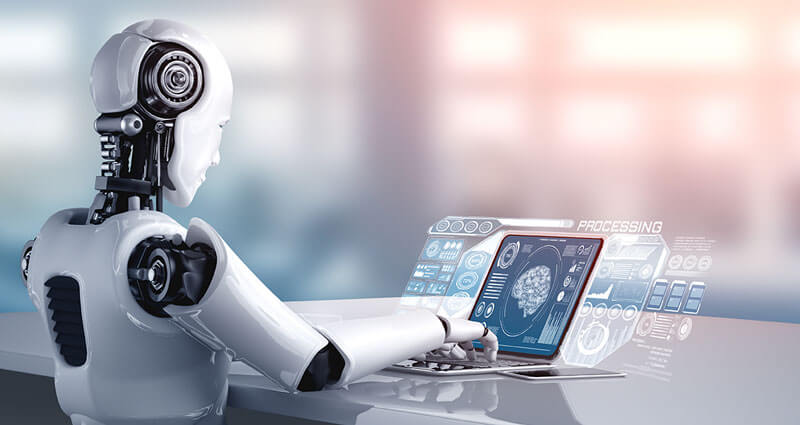
\includegraphics[width=\paperwidth,height=\paperheight]{supervised-vs-unsupervised-learning.jpg}}
	\begin{frame}[plain]
			% Contenu du frame
	
		\titlepage
		
\includegraphics[scale=0.3]{BensearchLogo-removebg-preview.png}\hfill
		%	
\includegraphics[scale=0.7]{images}\hfill
			
\includegraphics[scale=0.2]{bensearch.png}	
	\end{frame}
}

\section{Introduction à l'IA et au Machine Learning}
\subsection{Qu'est ce que l'IA?}
\subsection{Qu'est ce que le Machine Learning?}
\subsection{Difference entre le Machine Learning et l'IA}
\subsection{Histoire de l'IA}
\subsection{Approches techniques de l'IA}
\subsection{L'IA en robotique}
\subsection{Introduction au Big Data et son intégration avec l'IA}
\subsection{Concepts de base de l'apprentissage automatique}
\subsection{Types de Machine Learning}
\subsection{Travailler avec les données}
\subsection{Préparation des données pour l'apprentissage automatique}

{
	\setbeamertemplate{background}{
\includegraphics[width=\paperwidth,height=\paperheight]{ia_ml.jpg}}
\begin{frame}[plain]{Artificial Intelligence and Machine Learning 1}
%	\centering
%
\includegraphics[width=\linewidth]{ia_ml.jpg}
\end{frame}
}	% Page de titre
	%\begin{frame}
	%		\titlepage
	%\end{frame}

	%	\frametitle{Questions clés pour comprendre l'impact quotidien de l'IA}
	%\section{Artificial Intelligence and Machine Learning 1}
	\section{Introduction à l'IA et au Machine Learning}
\begin{frame}
	\frametitle{Introduction à l'IA et au Machine Learning}
	\begin{itemize}
		\item Qu'est ce que l'IA?
		\item Histoire de l'IA
		\item Machine Learning
		\item L'IA en robotique
		\item Introduction au Big Data et son intégration avec l'IA
		%\item Concepts de base de l'apprentissage automatique
		%\item Types d'apprentissage automatique
		\item Éviter les pièges et travailler avec les données
		\item Principes du Machine Learning
		\item Avantages et inconvénients de l'IA et du ML
		\item Conclusion 
	\end{itemize}
\end{frame}

\subsection{Qu'est ce que l'IA?}
\begin{frame}{Questions clés pour comprendre l'impact quotidien de l'IA}
	
	\begin{figure}[h]
		\centering
		\begin{minipage}{0.48\textwidth}
			\centering
			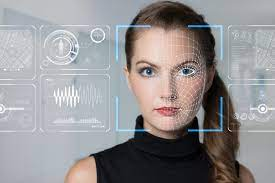
\includegraphics[width=\linewidth]{rf.jpeg}
			\caption{Reconnaissance faciale}
		\end{minipage}\hfill
		\begin{minipage}{0.48\textwidth}
			\centering
			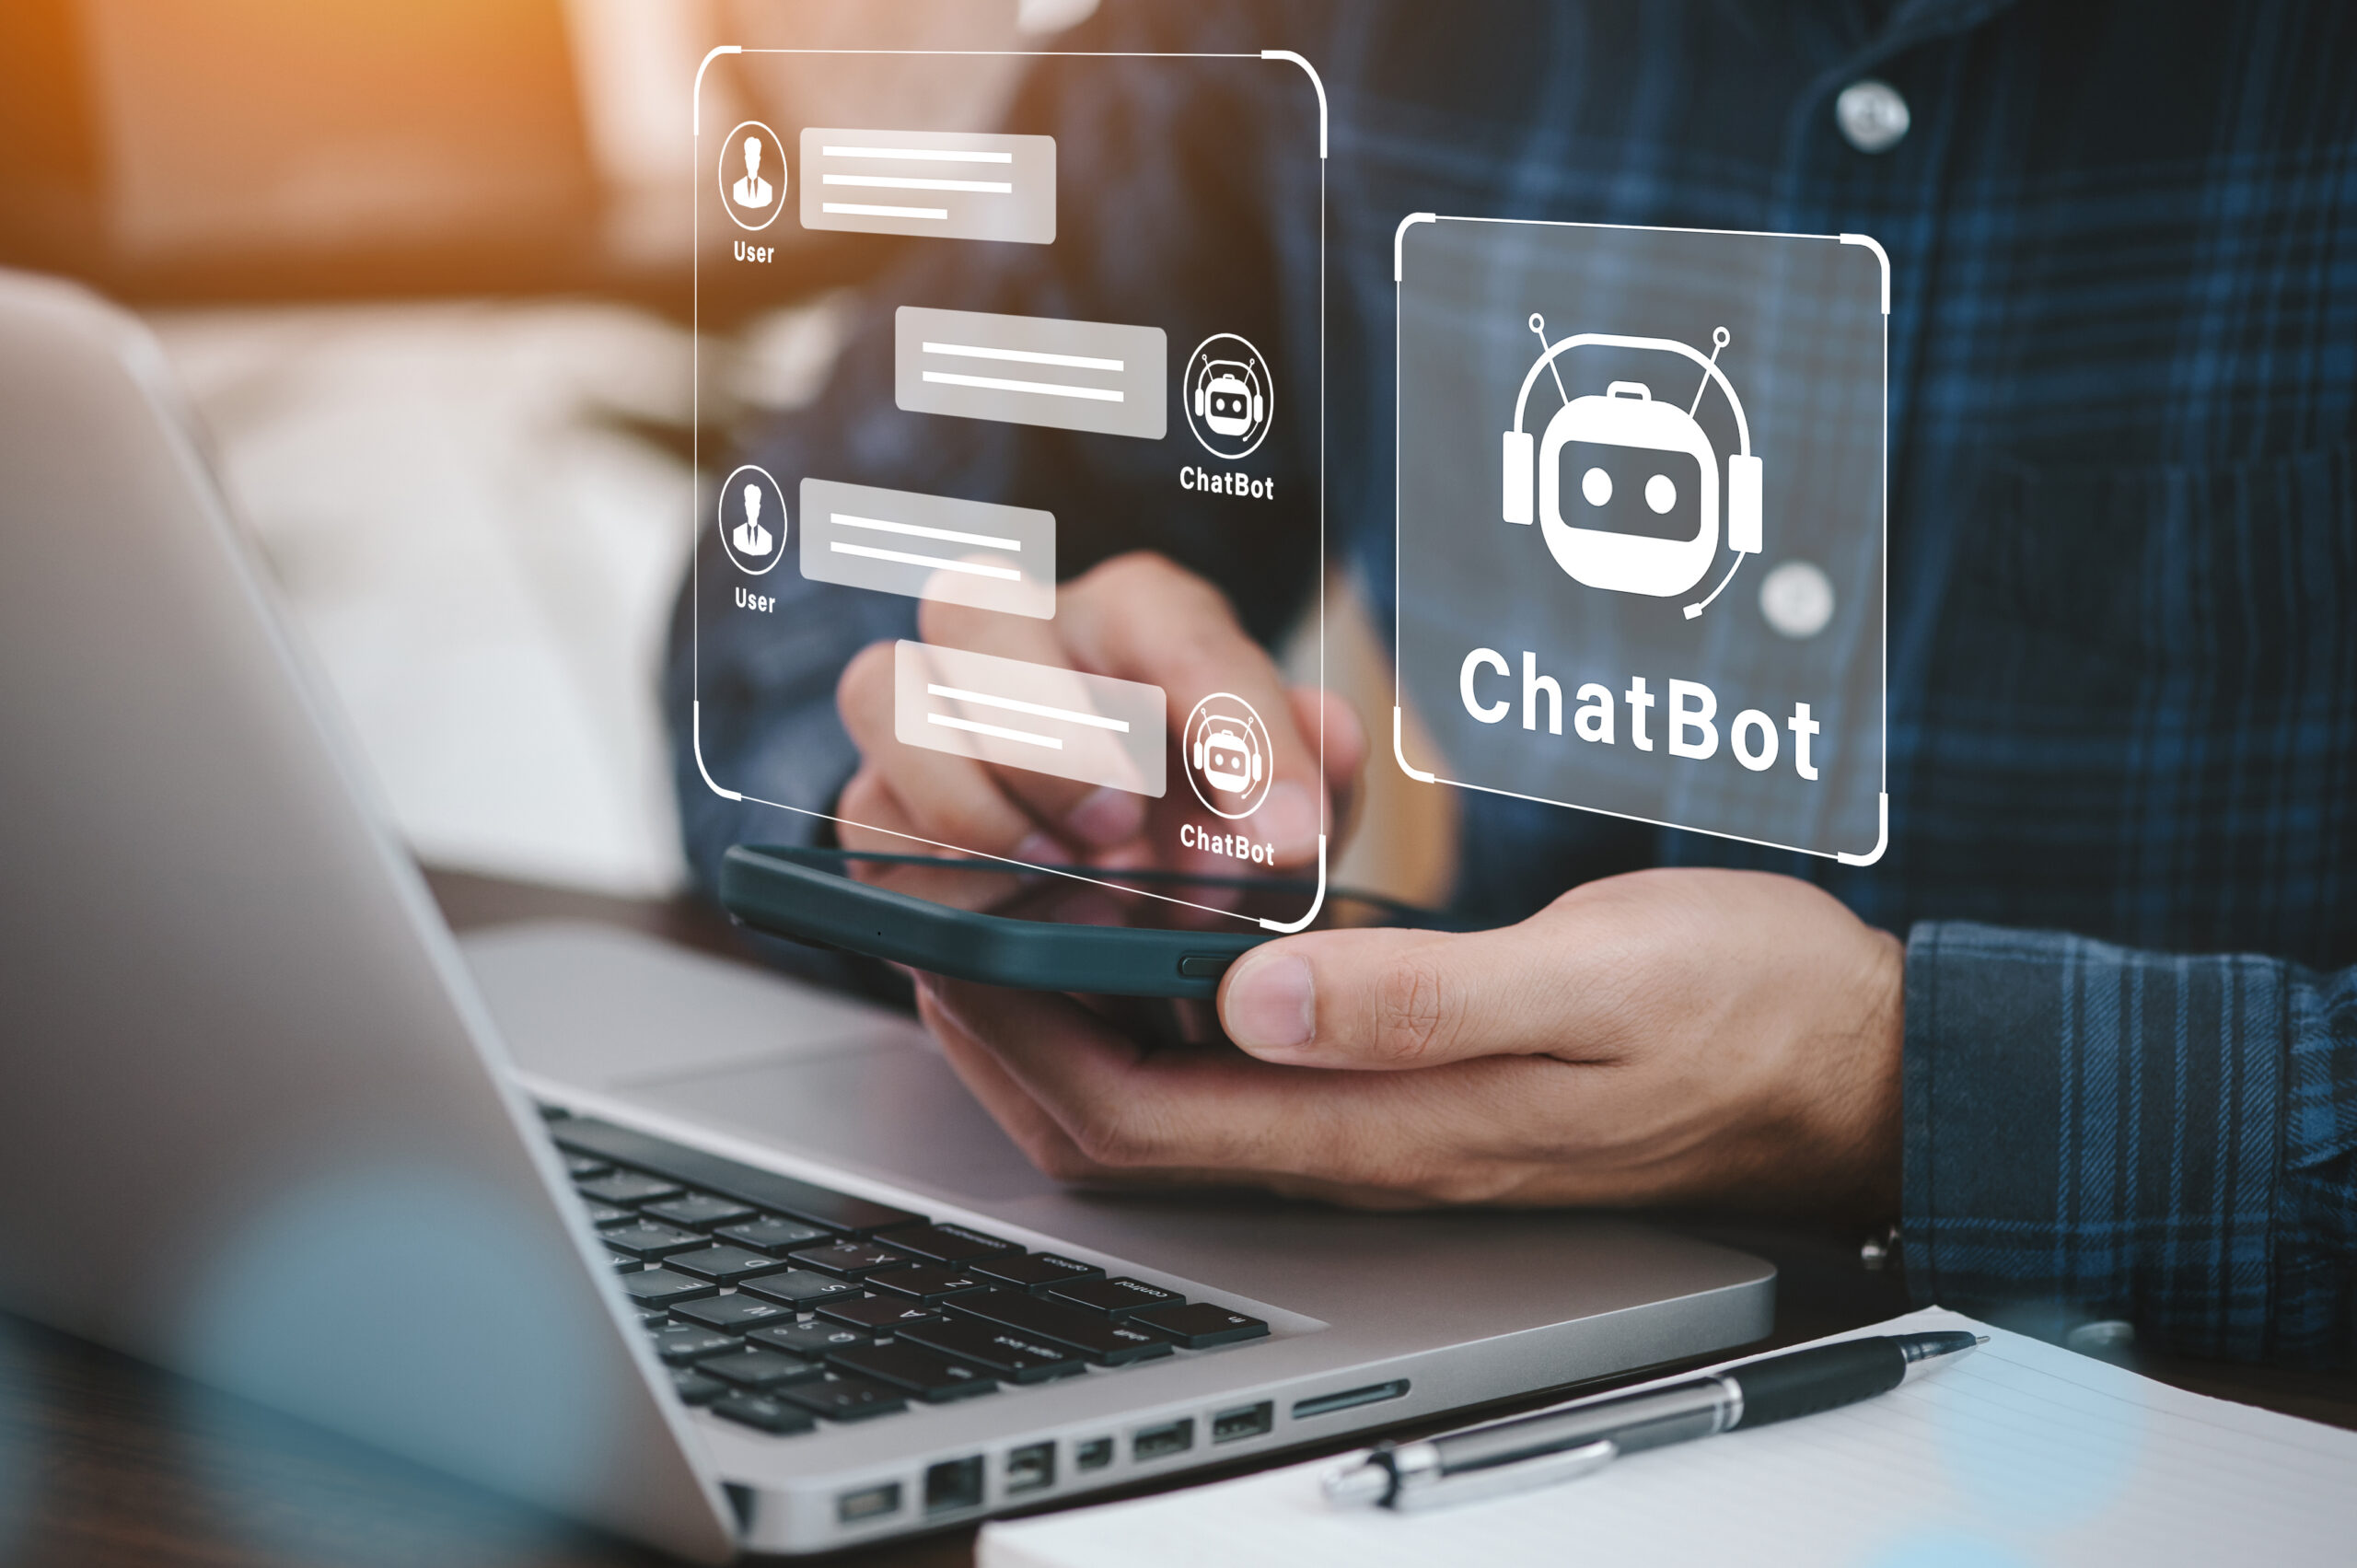
\includegraphics[width=\linewidth]{ChatBot.jpg}
			\caption{Application de chatbot}
		\end{minipage}

	\end{figure}
\end{frame}


\begin{frame}{Questions clés pour comprendre l'impact quotidien de l'IA}
\begin{figure}
	\begin{minipage}{0.48\textwidth}
	\centering
	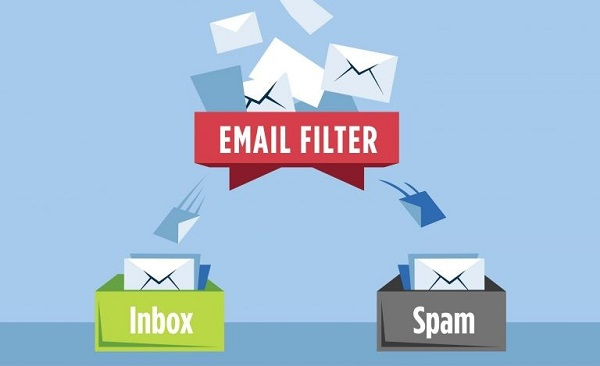
\includegraphics[width=\linewidth]{spam-1.jpg}
	\caption{Classification d'emails}
\end{minipage}\hfill
\begin{minipage}{0.44\textwidth}
	\centering
	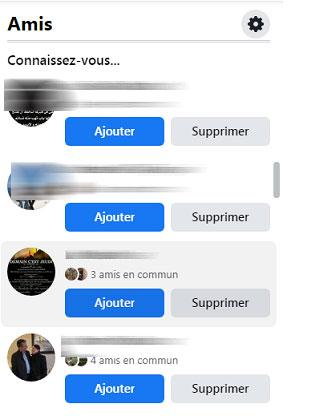
\includegraphics[width=\linewidth]{connaissez-vous-facebook.jpg}
	\caption{Suggestion d'amis facebook}
\end{minipage}
\end{figure}
\end{frame}
	%	\begin{itemize}
		%	\item Comment les systèmes de recommandation personnalisée fonctionnent-ils pour suggérer des produits, des films ou de la musique adaptés à nos préférences ?
	%		\item Comment les voitures autonomes sont-elles capables de détecter et de réagir aux obstacles sur la route de manière autonome ?
	%		\item Comment les applications de traduction instantanée parviennent-elles à convertir automatiquement un texte d'une langue à une autre ?
	%		\item Comment les assistants virtuels, tels que Siri ou Google Assistant, comprennent-ils nos commandes vocales et fournissent-ils des réponses pertinentes ?
	%		\item Comment les moteurs de recherche sont-ils en mesure de fournir des résultats personnalisés et pertinents en fonction de notre historique de recherche ?
	%		\item Comment les systèmes de reconnaissance faciale sont-ils capables d'identifier et de reconnaître les visages dans les photos ou les vidéos ?
	%		\item Comment les applications de chatbot utilisent-elles l'apprentissage automatique pour comprendre et répondre aux questions des utilisateurs de manière conversationnelle ?
		%	\item Comment les systèmes de détection de fraude analysent-ils les modèles d'activité pour identifier les transactions suspectes ?
		%	\item Comment les filtres anti-spam des boîtes e-mail sont-ils capables de trier les messages indésirables des messages légitimes ?
	%		\item Comment les applications de reconnaissance vocale transforment-elles nos paroles en texte de manière précise et rapide ?
	%	\end{itemize}

		
	\begin{frame}
		\frametitle{Questions clés pour comprendre l'impact quotidien de l'IA}
		
		\begin{figure}[h]
			\centering
			\begin{minipage}{0.5\textwidth}
				\centering
				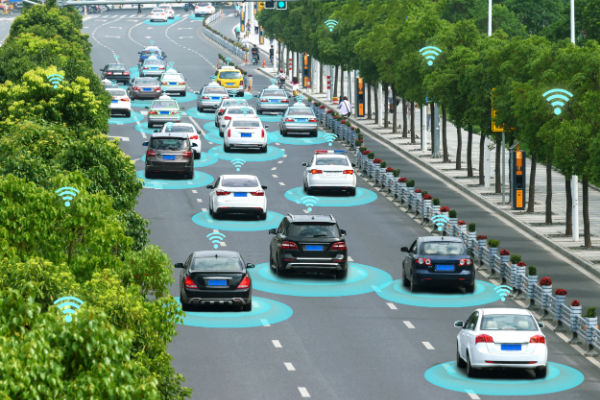
\includegraphics[width=\linewidth]{voiture-autonome.jpg}
				\caption{Voiture autonome}
			\end{minipage}\hfill
			\begin{minipage}{0.5\textwidth}
				\centering
				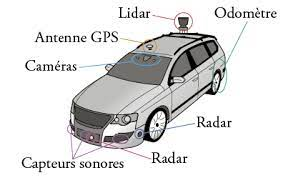
\includegraphics[width=\linewidth]{voitureauto.jpeg}
				\caption{Composantes }
			\end{minipage}
		\end{figure}
	Comment les voitures autonomes sont-elles capables de détecter et de réagir aux obstacles sur la route de manière autonome ?
		
	\end{frame}	
		
		
	\begin{frame}{Questions clés pour comprendre l'impact quotidien de l'IA}
		
		\begin{figure}[h]
			\centering
			\begin{minipage}{0.4\textwidth}
				\centering
				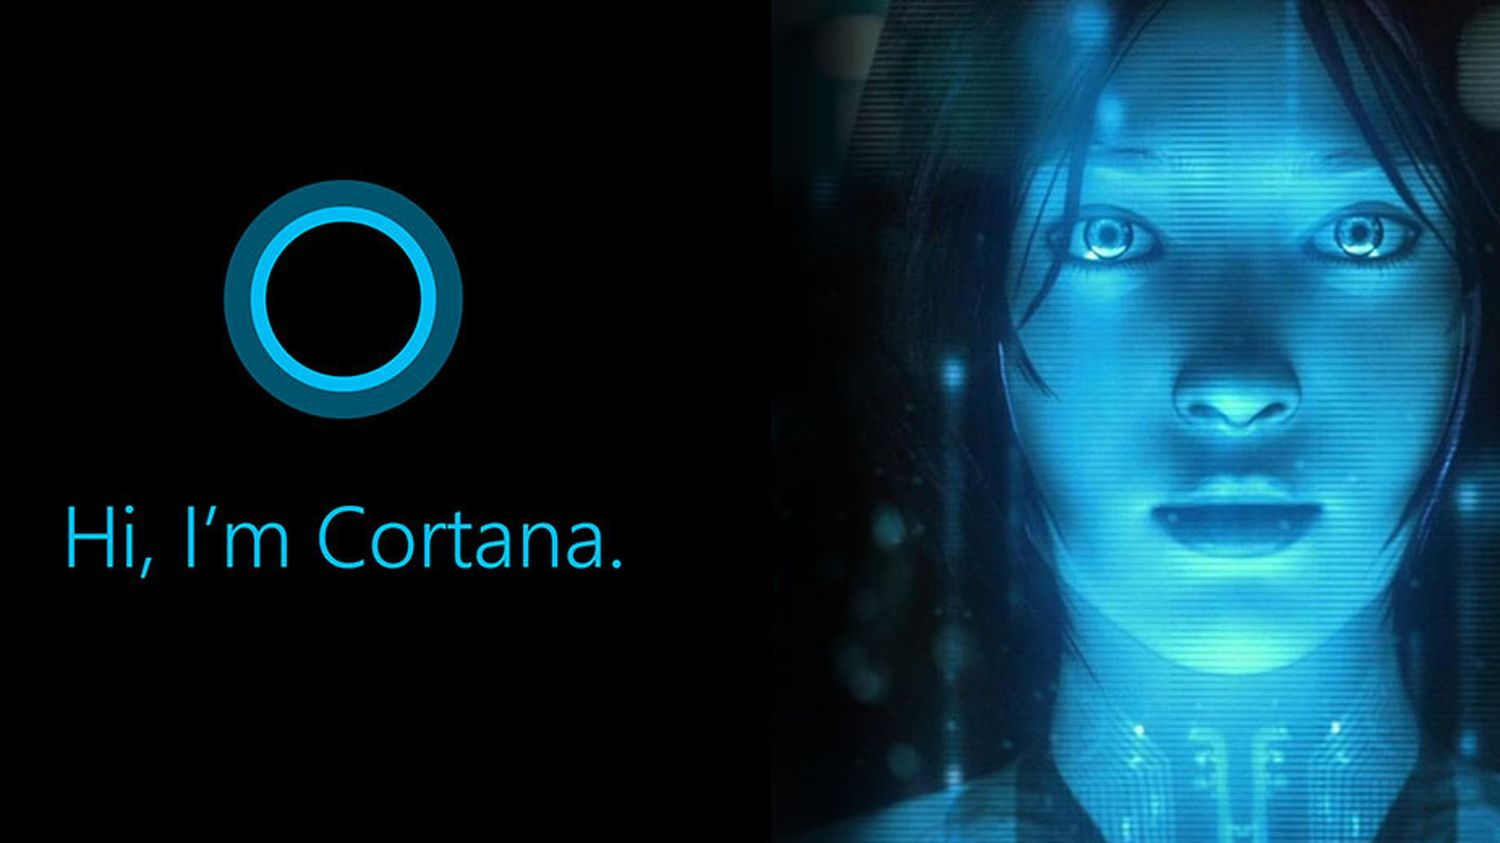
\includegraphics[width=\linewidth]{cortana_.jpg}
				\caption{Assistant personnel intelligent de MS}
			\end{minipage}\hfill
			\begin{minipage}{0.34\textwidth}
				\centering
				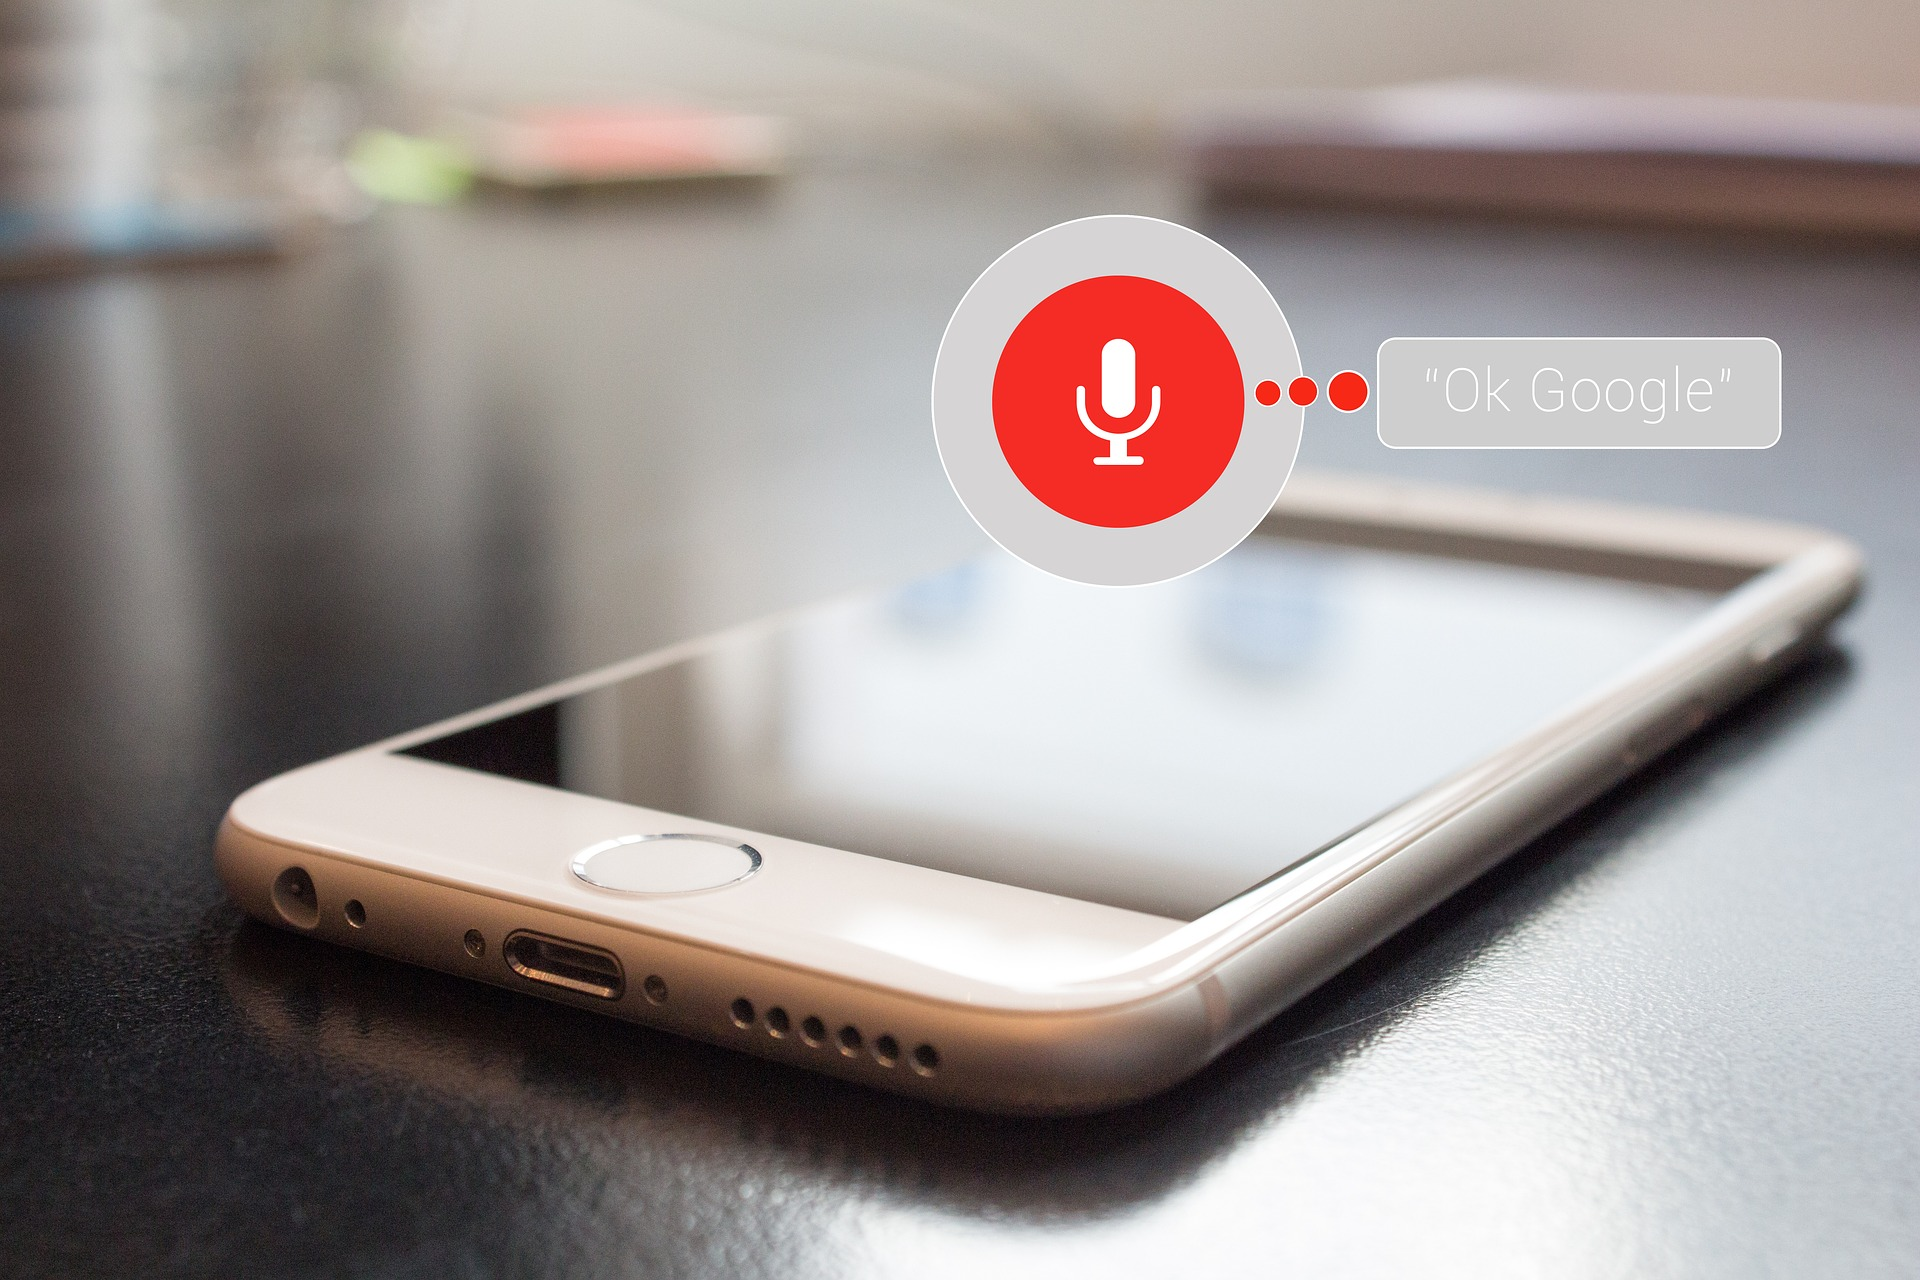
\includegraphics[width=\linewidth]{voice-control.jpg}
				\caption{Applications de reconnaissance vocale}
			\end{minipage}
			\vspace{0.5cm}
			\begin{minipage}{0.4\textwidth}
				\centering
				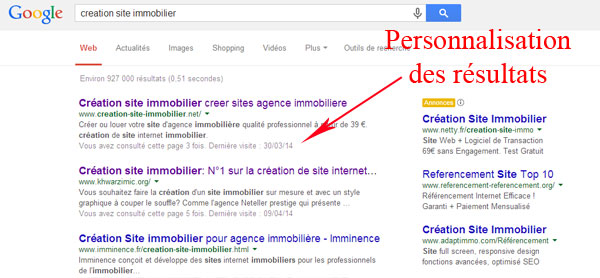
\includegraphics[width=\linewidth]{personnalisation.jpg}
				\caption{Resultat de recherche personalisée}
			\end{minipage}\hfill
			\begin{minipage}{0.32\textwidth}
				\centering
				
\includegraphics[width=\linewidth]{googlet.jpg}
				\caption{Application de traduction instantanée}
			\end{minipage}
		\end{figure}
		
	\end{frame}	
		


{
	\setbeamertemplate{background}{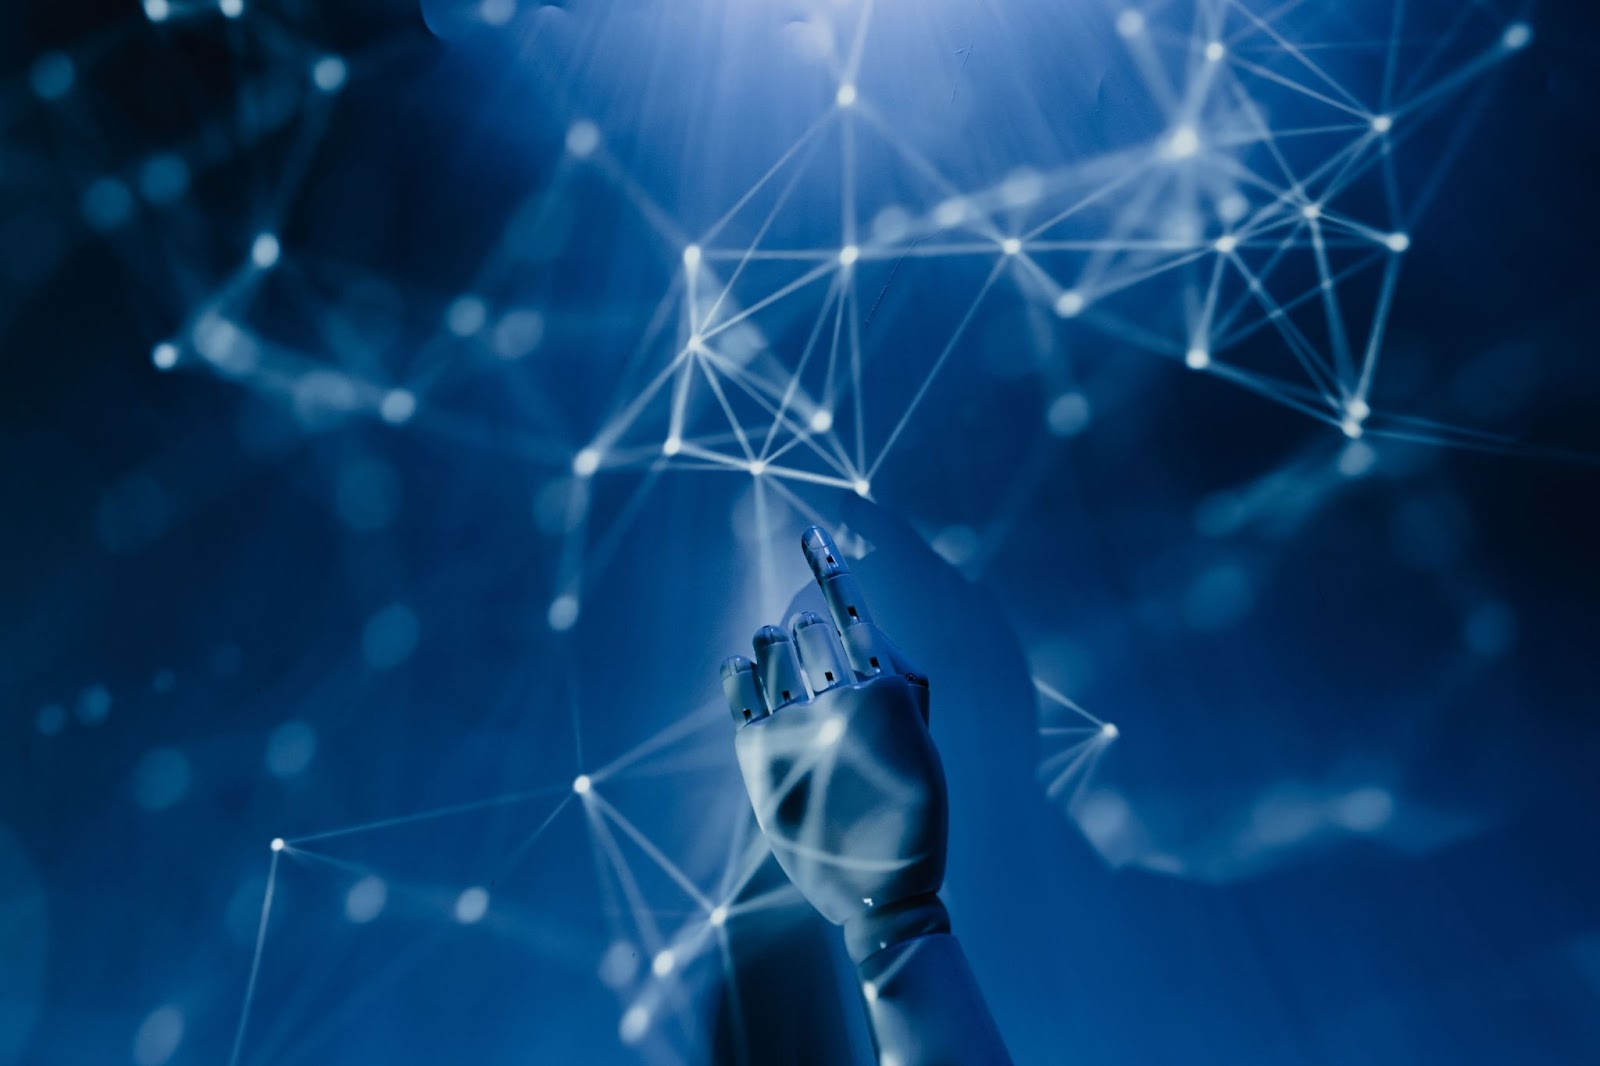
\includegraphics[width=\paperwidth,height=\paperheight]{bakiadef.jpeg}}
\begin{frame}
	\frametitle{Définition de l'IA selon quelques auteurs}
	\begin{itemize}
\color{white}		\item \textbf{John McCarthy (1956)} : "L'IA est la science et l'ingénierie de la création de machines intelligentes, qui ont la capacité de réaliser des tâches qui nécessitent normalement l'intelligence humaine."
\vspace{0.3cm}
		\item \textbf{Stuart Russell et Peter Norvig (2009)} : "L'IA est le domaine de l'informatique qui traite de la création et de l'étude de machines qui peuvent effectuer des tâches qui, si elles étaient accomplies par des êtres humains, nécessiteraient de l'intelligence."
		\vspace{0.3cm}
		\item \textbf{Marvin Minsky (1968)} : "L'IA est la construction de programmes informatiques qui peuvent accomplir des tâches qui, lorsqu'elles sont accomplies par des personnes, demandent de l'intelligence."
	\end{itemize}
	
\end{frame}
}	% Slide 2: Introduction



	% Slide 3: Objectifs du projet
	\subsection{Histoire de l'IA}
	\begin{frame}{Les dates clés de l'Intelligence Artificielle}
		\centering
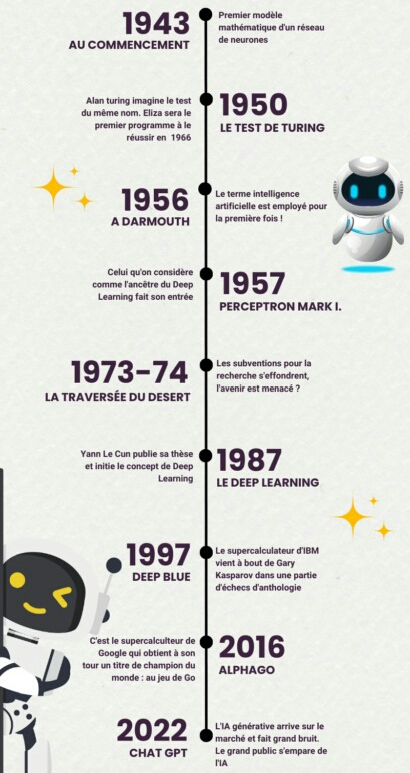
\includegraphics[width=0.6\linewidth]{AIhistory.jpeg}
%\caption{Les dates clés de l'Intelligence Artificielle}
	\end{frame}

%	\subsection{Histoire de l'IA}
\begin{frame}{Les dates clés de l'Intelligence Artificielle}
	\centering
	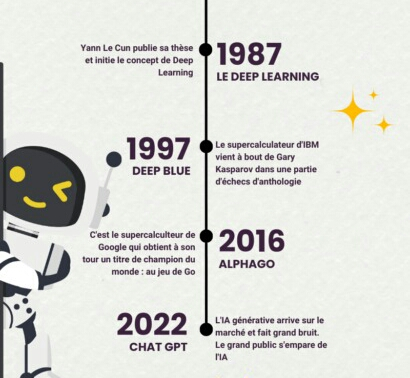
\includegraphics[width=0.6\linewidth]{hia.jpeg}
	%\caption{Les dates clés de l'Intelligence Artificielle}
\end{frame}


\begin{frame}{Les Intelligences Artificielles populaires }
	\centering
	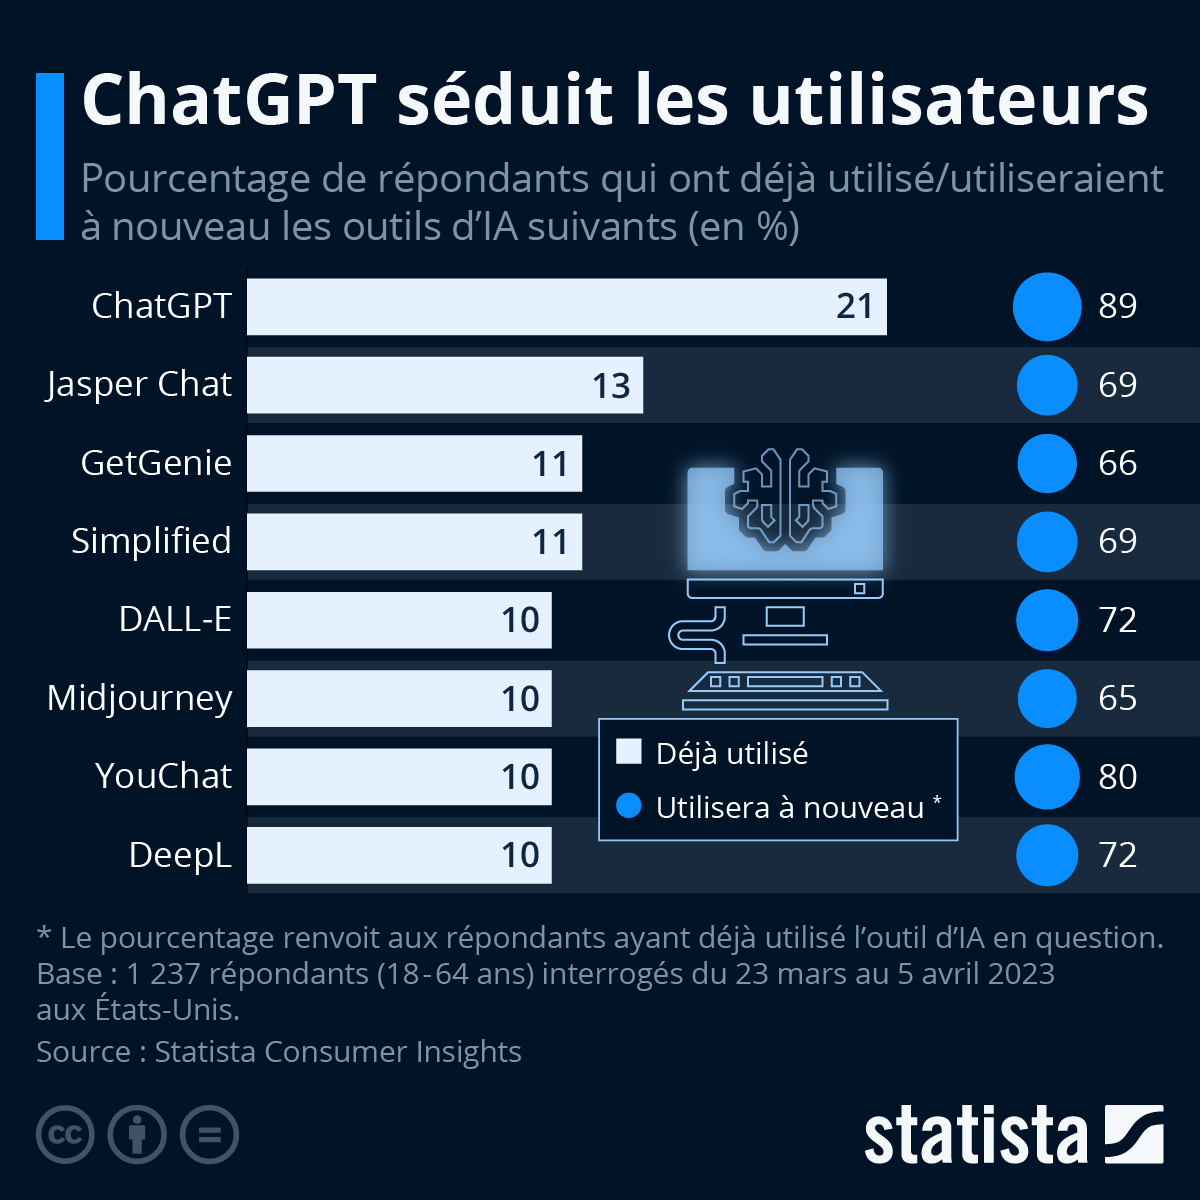
\includegraphics[width=0.6\linewidth]{PopularAI.jpeg}
	%\caption{Les dates clés de l'Intelligence Artificielle}
\end{frame}


\begin{frame}{La course vers les brevets}
	\centering
	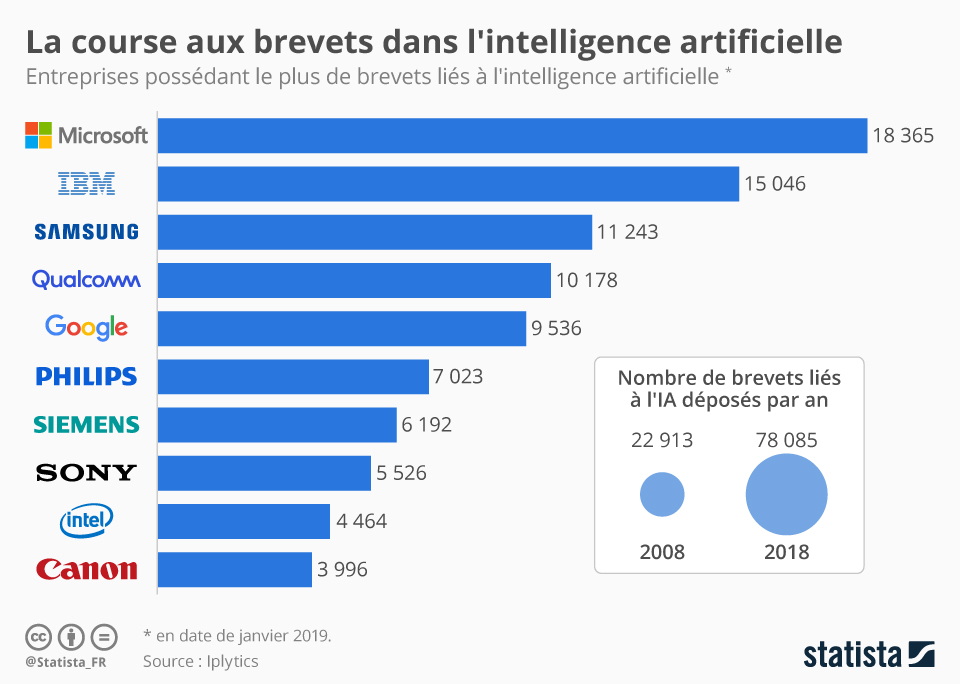
\includegraphics[width=\linewidth]{BrevetIA.jpeg}
	%\caption{Les dates clés de l'Intelligence Artificielle}
\end{frame}


\begin{frame}{Future de l'IA}
	\centering
	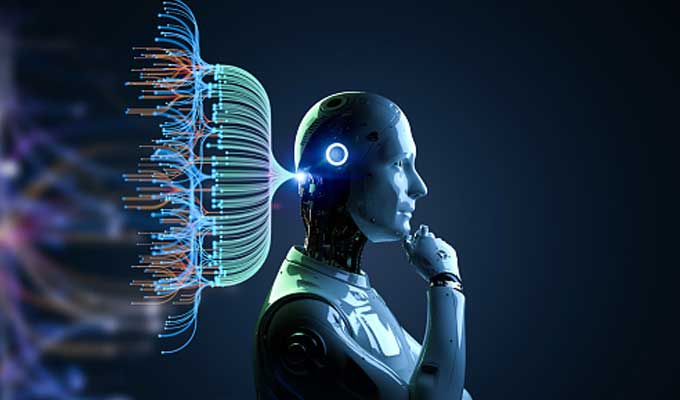
\includegraphics[width=\linewidth]{Fut.jpg}
	%\caption{Les dates clés de l'Intelligence Artificielle}
\end{frame}

\subsection{Qu'est ce que le Machine Learning?}
		\begin{frame}{Qu'est ce que le Machine Learning}
	
	C'est tout processus par lequel un système améliore ses performances à partir de l'expérience issue des données.
	
	\centering
	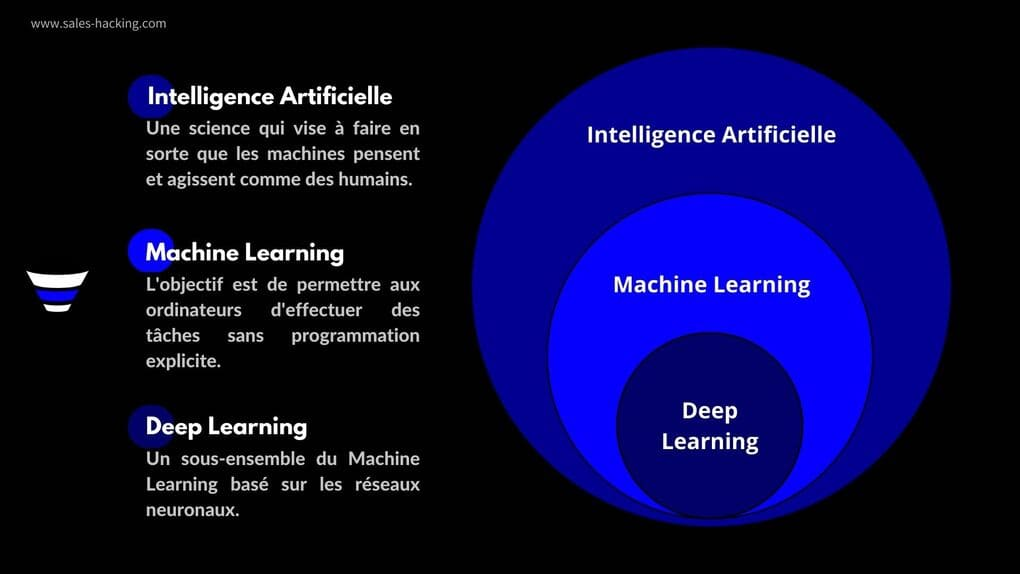
\includegraphics[width=\linewidth]{compar.png}
	%	\begin{block}{Différence entre l'IA et le Machine Learning}		
	\end{frame}

\subsection{Approches techniques de l'IA utilisées dans le ML}
\begin{frame}{Approches techniques de l'IA utilisées dans le ML}
	\centering
	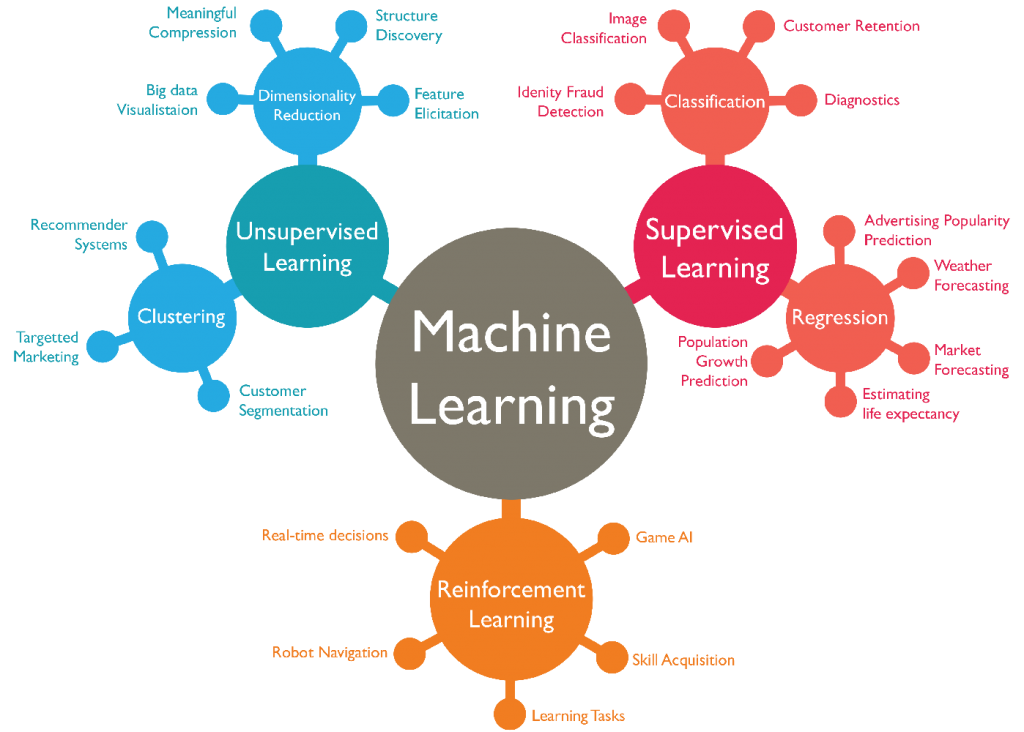
\includegraphics[width=0.9\linewidth]{tml.png}
\end{frame}


{
	\setbeamertemplate{background}{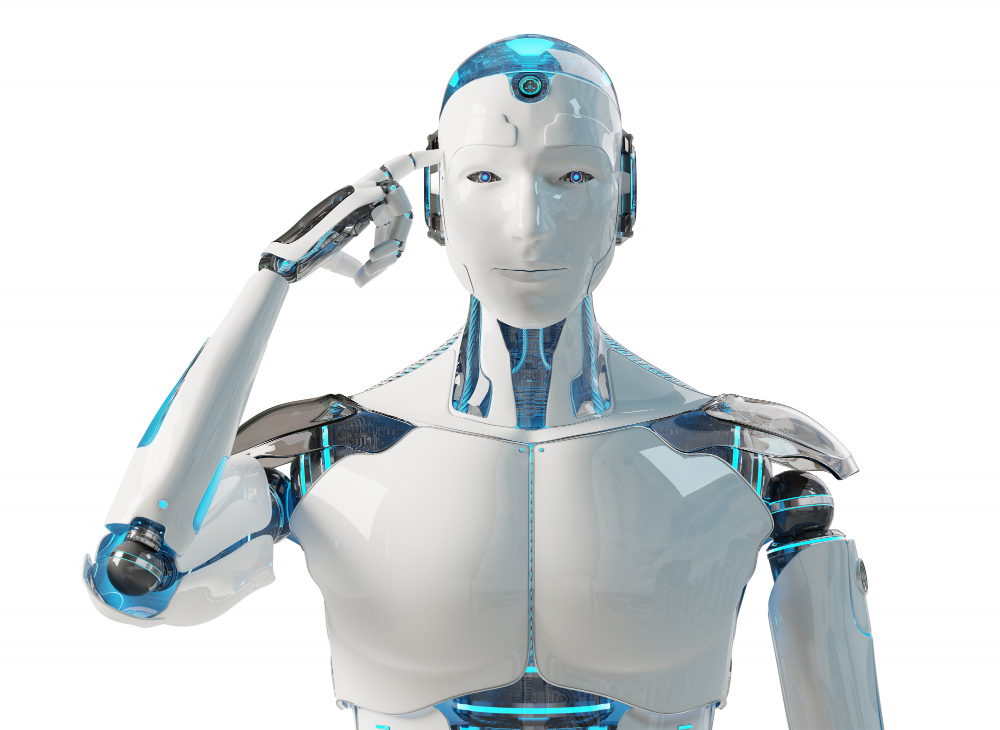
\includegraphics[width=\paperwidth,height=\paperheight]{white-male-cyborg-thinking-touching-his-head.jpg}}
\subsection{L'IA en robotique}
\begin{frame}{L'IA en robotique}
	\Large
	\begin{itemize}
		\item Applications de l'IA en robotique
		\item Exemples de robots intelligents
		\item Les défis de l'IA en robotique
	\end{itemize}
\end{frame}
}

\subsection{Applications de l'IA en robotique}
\begin{frame}{Applications de l'IA en robotique}
    \begin{itemize}
	\item Industrie : robot de gestion de chaîne d'assemblage...
	\item Armée : drone, robot-espion, robot-mule...
	\item Sécurité : vidéosurveillance...
	\item Santé : échographie, chirurgie assistée...
	\item Aérospatial : robot explorateur de la NASA...
	\item Transport : voiture autonome...
	\item Usage domestique : robot aspirateur, robot tondeuse...
	\item Accompagnement : jouet automatisé, robot humanoïde...
	\item Informatique : chatbot, assistant vocal...
\end{itemize}
\end{frame}

\begin{frame}{Exemples de Robots intelligents}
	\begin{itemize}
		\item Atlas : Robot humanoïde développé par Boston Dynamics, connu pour sa mobilité et sa dextérité avancées.
		\item Asimo : Robot humanoïde développé par Honda, célèbre pour sa marche bipède, sa capacité à monter les escaliers et ses mouvements semblables à ceux d'un humain.
		\item iCub : Robot humanoïde à source ouverte conçu pour étudier la cognition et le développement humains.
		\item Nao : Petit robot humanoïde créé par SoftBank Robotics, utilisé dans l'éducation, la recherche et le divertissement, capable d'interagir avec les humains par la parole et les gestes.
	\end{itemize}
\end{frame}

\frame[plain]
{
	\centering
	
	\movie[width=10cm,height=7.5cm,poster]{}{AtlasGetsGripBostonDynamics.mp4}
	
}






\begin{frame}[plain]
	\centering
	\includemedia[
	width=10cm,
	height=7.5cm,
	addresource=Robotshumanoïdes.mp4,
	flashvars={source=Robotshumanoïdes.mp4}
	]{}{VPlayer.swf}
\end{frame}

% Slide 6: Parties prenantes
\section{Le Big Data et son intégration avec l'IA}
\subsection{Qu'est-ce que le Big Data ?}
\begin{frame}
	\frametitle{Le Big Data et son intégration avec l'IA}
	
	\begin{itemize}
		\item Les Big Data sont les traces numériques (données) qui se génèrent dans l'ensemble de l'écosystème numérique.
		\item Les Big Data sont des actifs d'information à haut volume, haute vélocité et haute variété.
		
		\item Les principales caractéristiques des Big Data sont les quatre V 
	\end{itemize}
	
	\begin{figure}
		\centering
		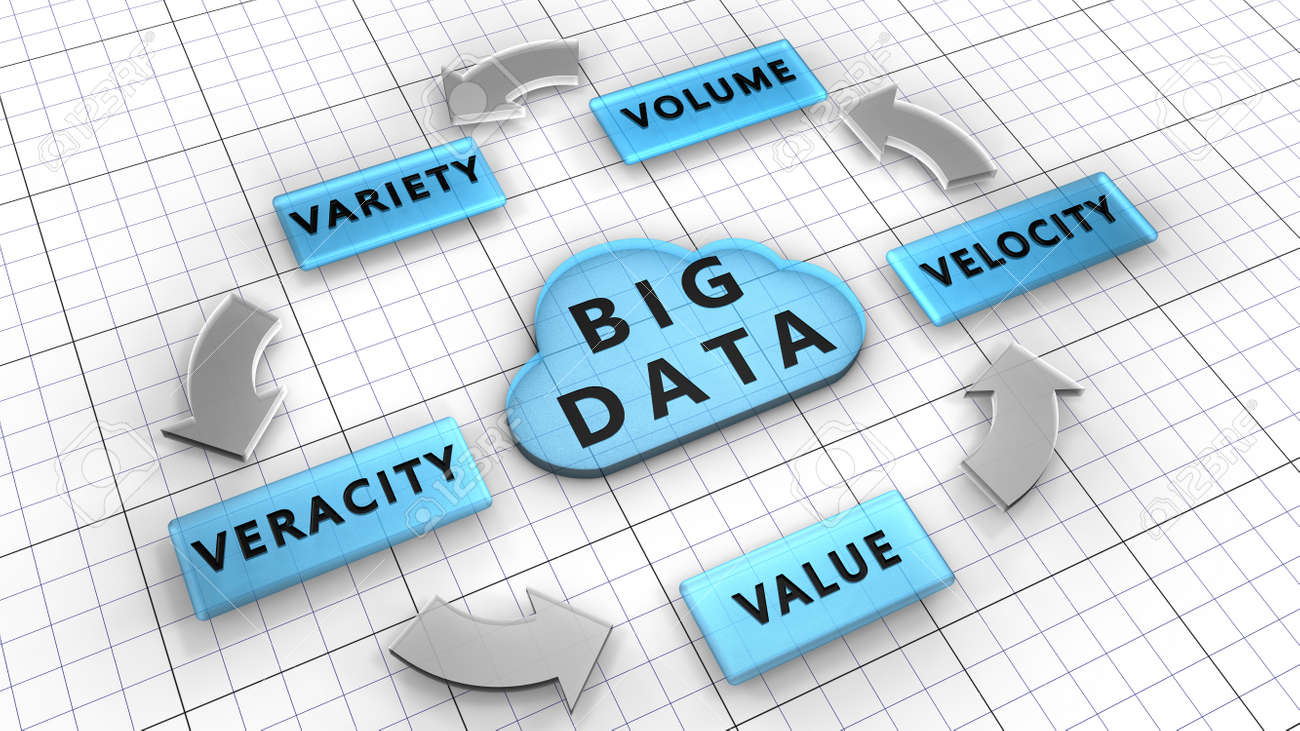
\includegraphics[width=0.6\textwidth]{bigDa.jpg}
	%	\caption{Illustration du concept de Big Data}
	\end{figure}
	
\end{frame}
\begin{comment}
		\begin{itemize}
		\item Qu'est-ce que le Big Data ?
		\item Les 4 V du Big Data (Volume, Vélocité, Variété, Véracité)
		\item Comment le Big Data alimente l'IA
	\end{itemize}
\end{comment}

\subsection{Impact des Big Data}

\begin{frame}
	\frametitle{Impact des Big Data}
	
	\begin{itemize}
		\item Les appareils IoT génèrent continuellement d'énormes volumes de données.
\item L'analyse des Big Data aide les entreprises à obtenir des informations à partir des données collectées par les appareils IoT.
	\end{itemize}
	
	\begin{figure}
		\centering
		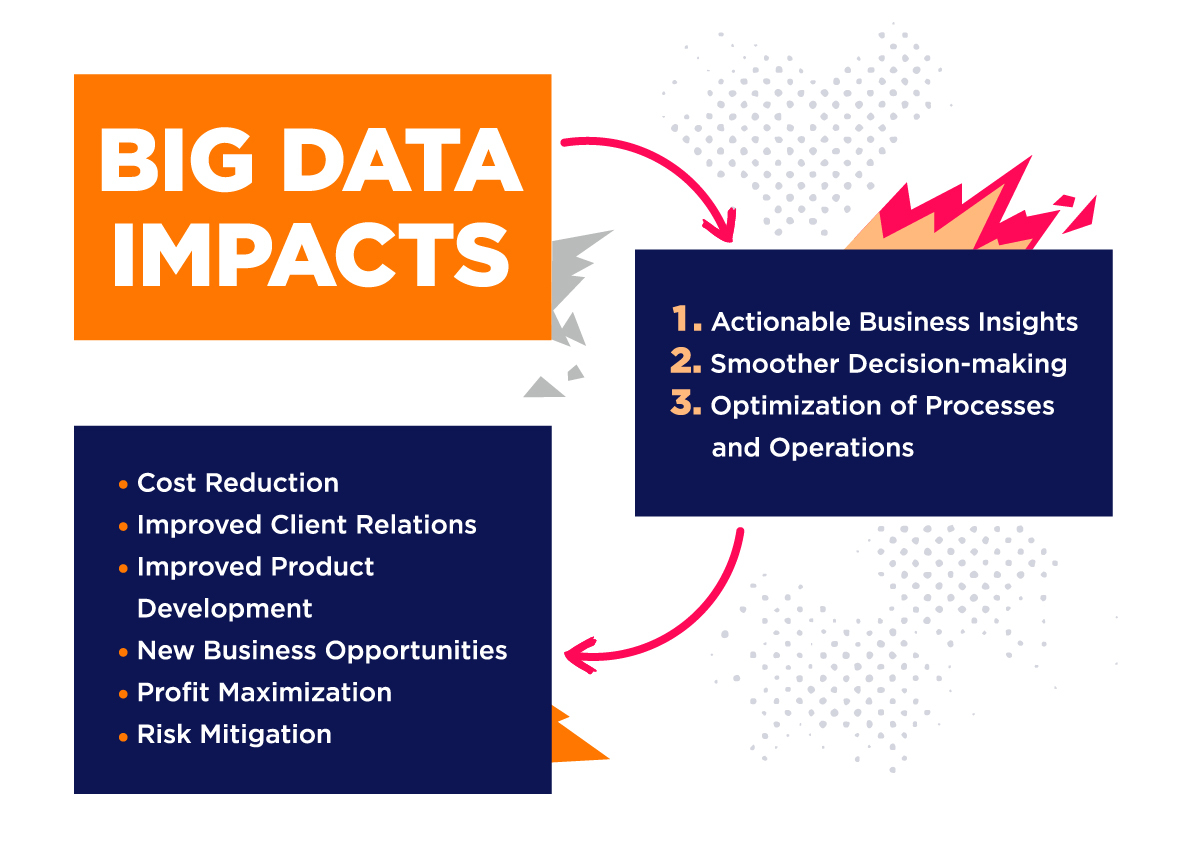
\includegraphics[width=0.6\textwidth]{big_data_benefits.jpg}
		%	\caption{Illustration du concept de Big Data}
	\end{figure}
	
\end{frame}






	\begin{frame}
	\frametitle{Comment le Big Data alimente l'IA?}
		\begin{figure}
		\centering
		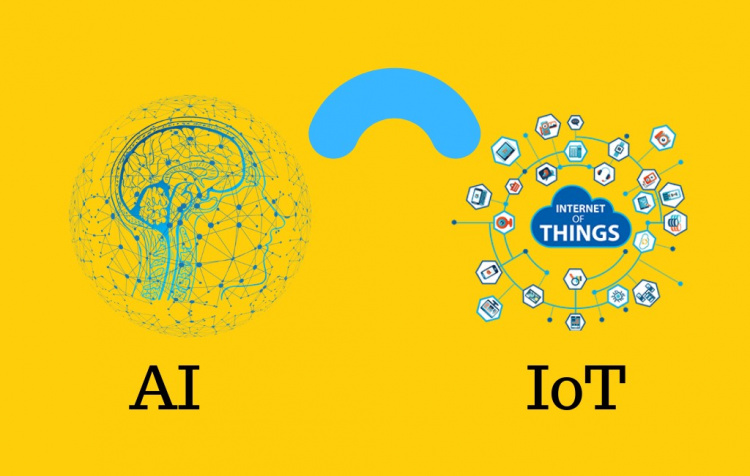
\includegraphics[width=0.6\textwidth]{ia-capteurs-iot.jpg}
		%	\caption{Illustration du concept de Big Data}
	\end{figure}
	\begin{itemize}
		\item Entraînement des modèles d'IA
		\item Amélioration de la précision
		\item Apprentissage en continu
		\item Détection des tendances et des modèles
		\item Personnalisation et recommandations
	\end{itemize}
\end{frame}



\begin{frame}
	\frametitle{Principe du Machine Learning}
	
	\begin{figure}
		\centering
		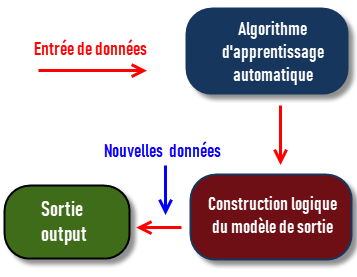
\includegraphics[width=0.5\textwidth]{ml-shema.png}
	\end{figure}
	
	\begin{enumerate}
		\item[\textcolor{blue}{1.}] \textcolor{blue}{Les influences majeures du ML}
		\item[\textcolor{blue}{2.}] \textcolor{blue}{Approche méthodologique du ML}
		\item[\textcolor{blue}{3.}] \textcolor{blue}{Types d'apprentissage statistique}
		\item[\textcolor{blue}{4.}] \textcolor{blue}{Travailler avec les données et éviter les pièges}
		\item[\textcolor{blue}{5.}] \textcolor{blue}{Quelques modèles de ML}
	\end{enumerate}
	
\end{frame}

\subsection{Les influences}
\begin{frame}{Les influences majeures du ML}
Le Machine learning ou apprentissage statistique est un champ d'étude de l'IA qui se fonde sur des approches statistiques pour donner aux ordinateurs la capacité d'apprendre à partir de données.\\


\begin{enumerate}
	\item La théorie formelle de la statistique
	\item L’accélération du développement des ordinateurs
	\item Le défi, dans de nombreux domaines, de corpus de données toujours plus grands
	\item L’accent mis sur la quantification dans une variété toujours plus large de disciplines
\end{enumerate}

\end{frame}
	\subsection{Méthodologie du ML}
	\begin{frame}{Resumé de la méthodologie}
		\begin{center}
			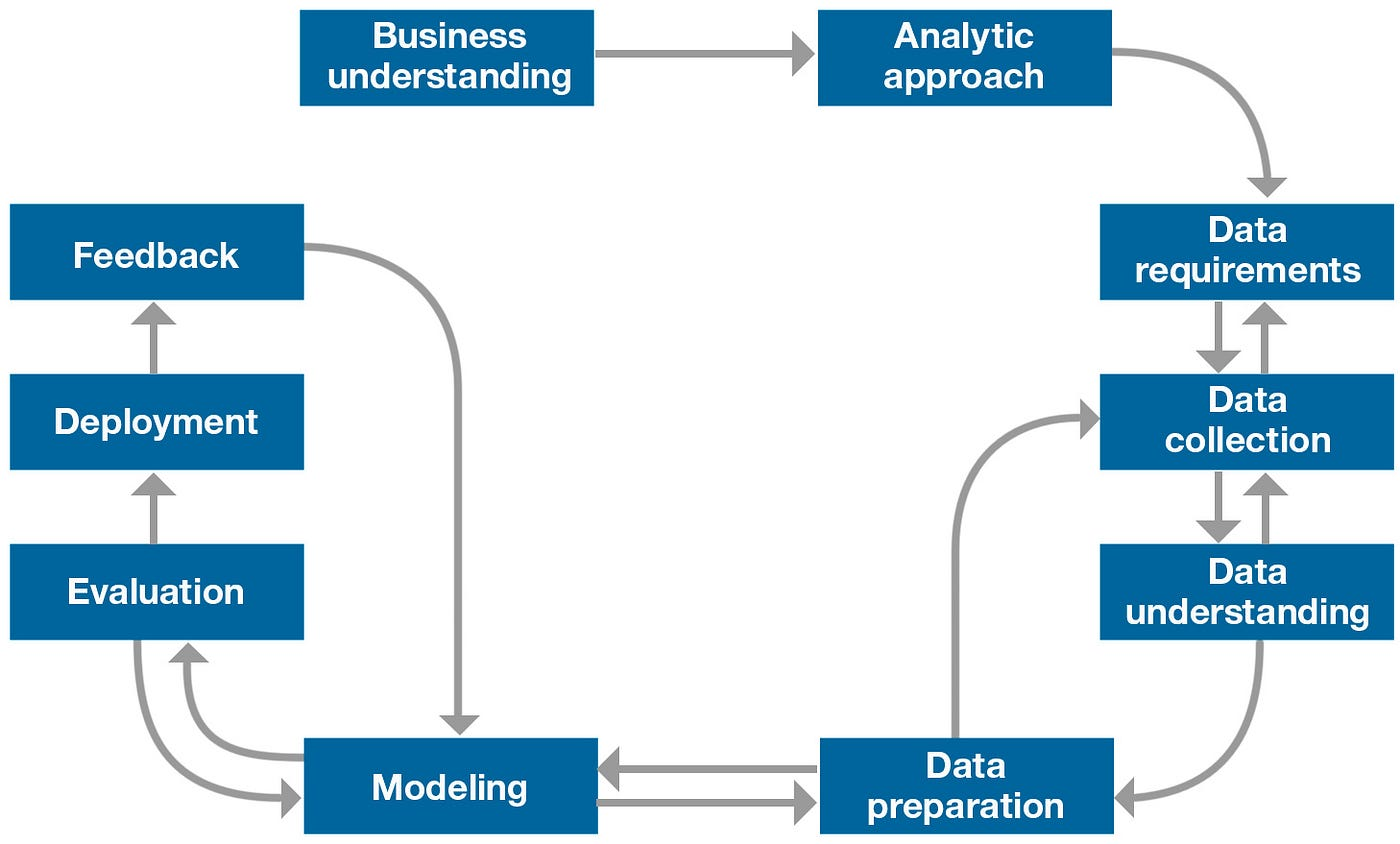
\includegraphics[scale=0.2]{DataMethod.jpg}
		\end{center}
	\end{frame}


	% Slide 5: Bénéfices attendus sysexpert.png




\subsection{Types d'apprentissages statistique}
\begin{frame}{Supervisé et non-supervisé}
\begin{itemize}
	\item Apprentissage supervisé
	\begin{itemize}
		\item Objectif : apprendre une fonction $f$ prédisant une variable $Y$ à partir de
		features $X$.
		\item Données : ensemble d'apprentissage $(X_i, Y_i)$
	\end{itemize}
 \item Apprentissage non-supervisé
 		\begin{itemize}
 			\item  Objectif: découvrir une structure au sein d'un ensemble d'individus $(X_i)$
 			\item Data : Learning set $(X_i)$
 		\end{itemize}
\end{itemize}
	\begin{figure}
	\centering
	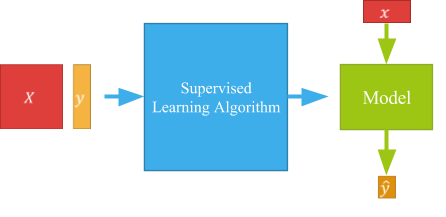
\includegraphics[width=0.6\textwidth]{Machine-Learning-3.png}
\end{figure}

\end{frame}


	\begin{frame}{Apprentissage supervisé}
	\centering
	\begin{figure}[h]
		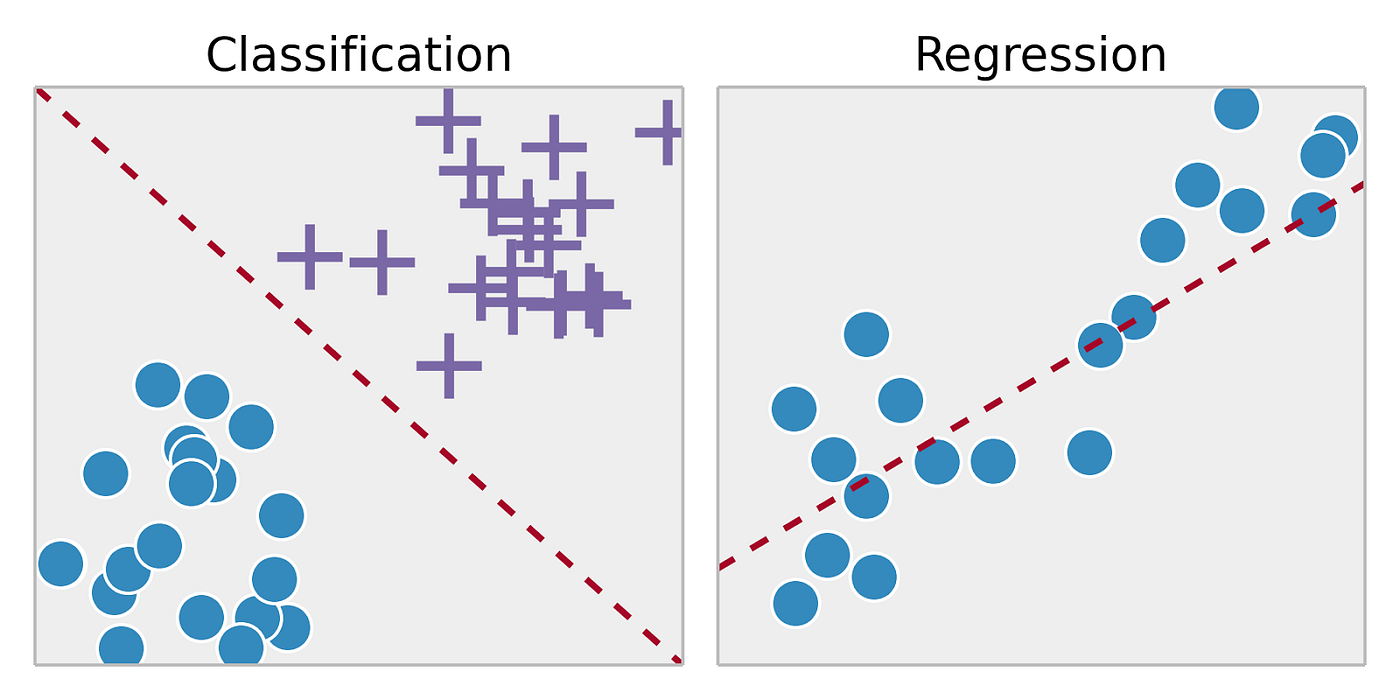
\includegraphics[width=\linewidth]{CR.png}
	%	\caption{Classification Vs Regression}
	\end{figure}
\end{frame}	



%	\setbeamertemplate{background}{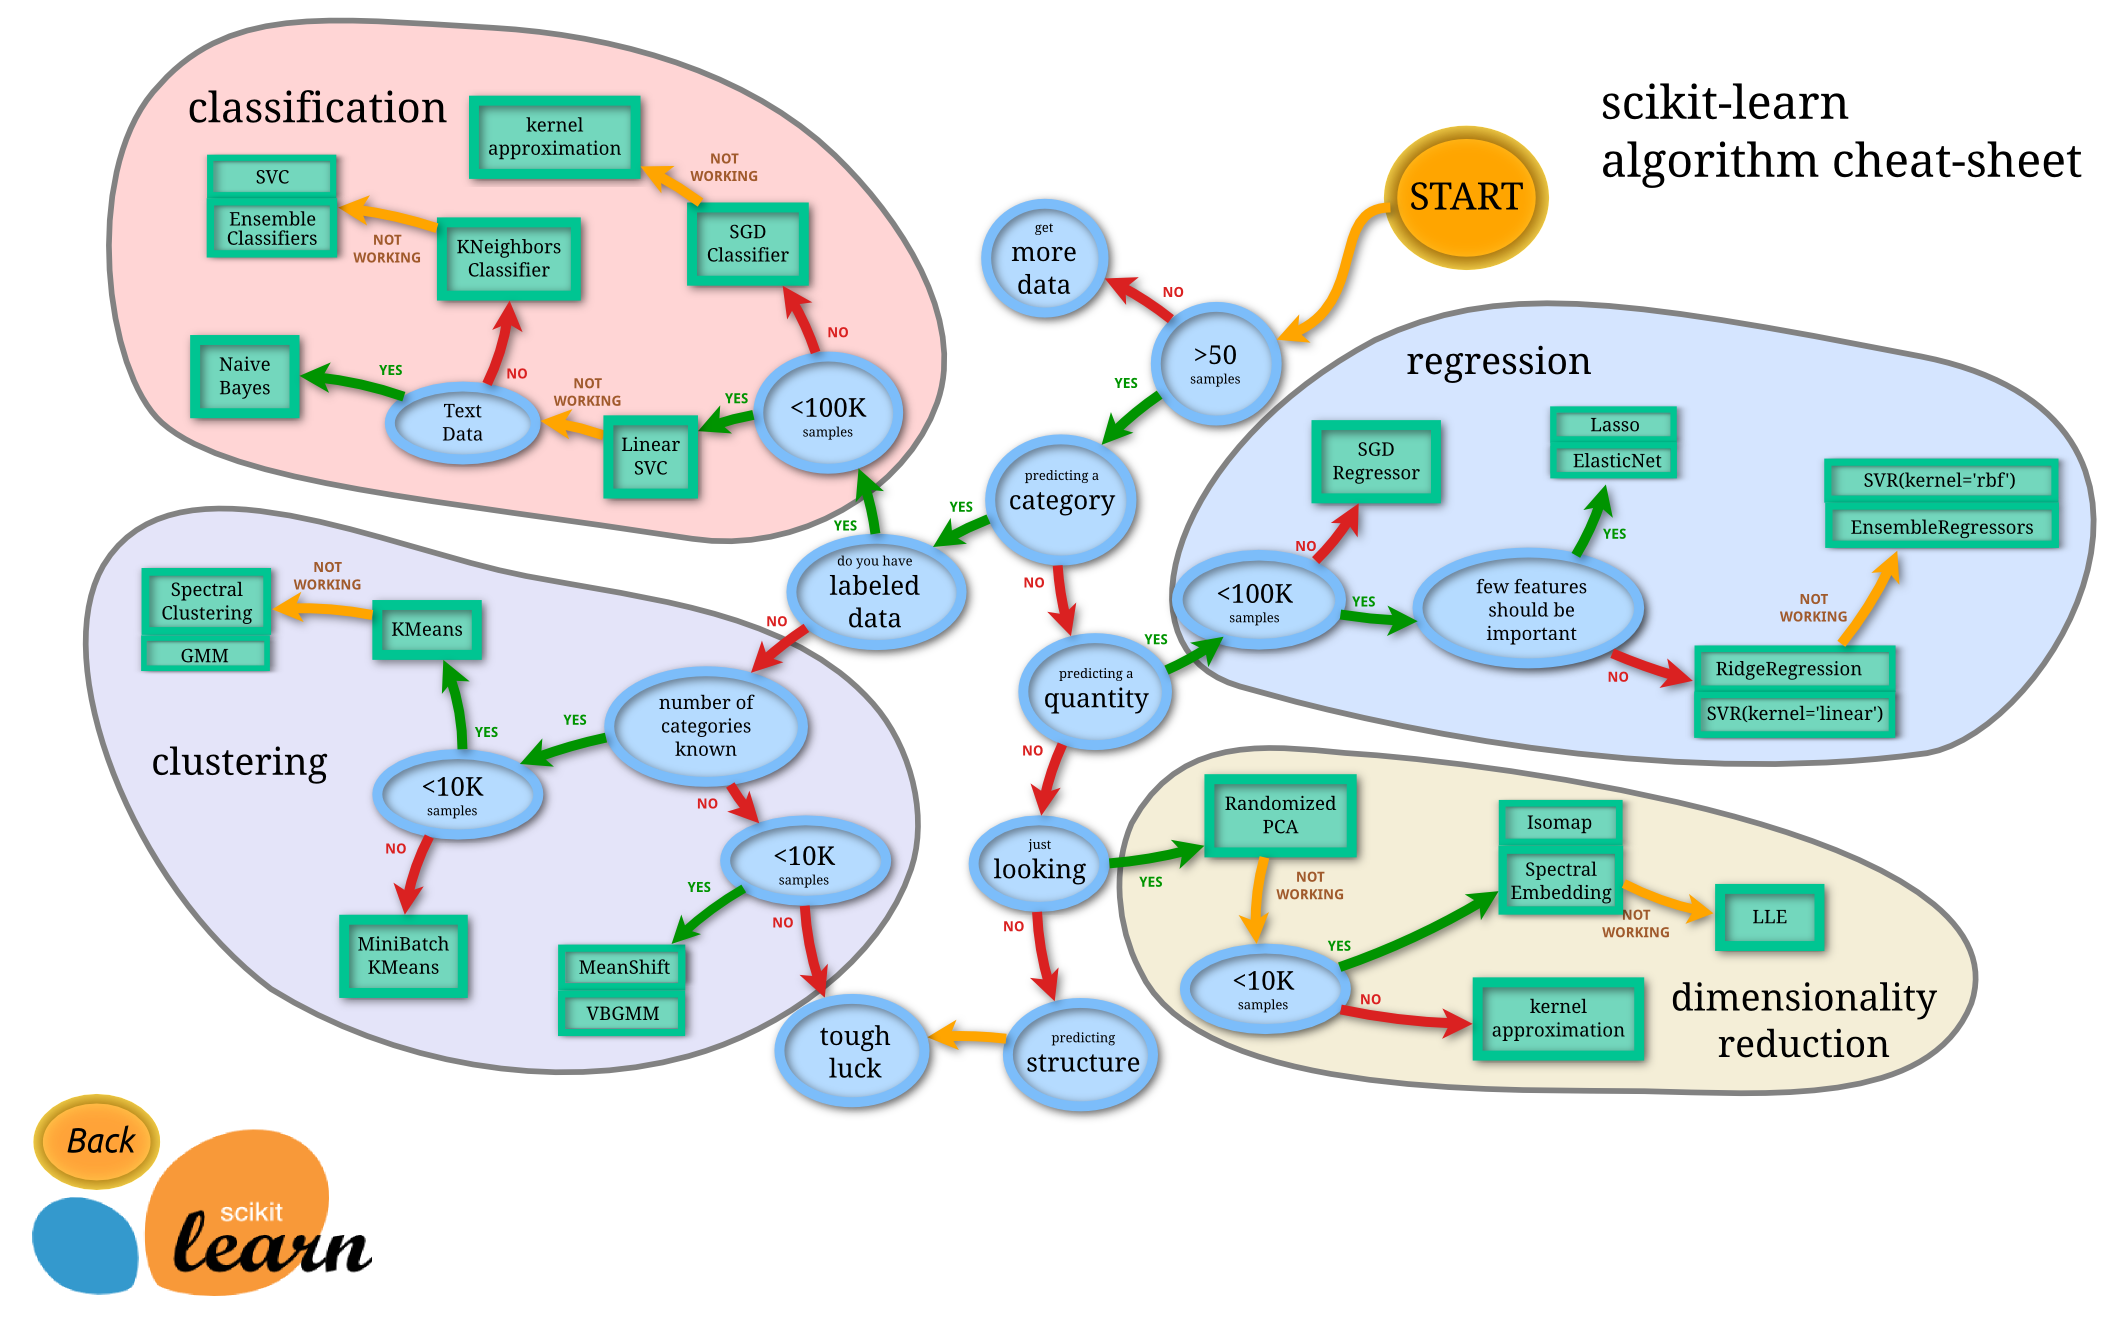
\includegraphics[width=\paperwidth,height=\paperheight]{ml_map.png}}
	\begin{frame}
					\centering
	\begin{figure}[h]
			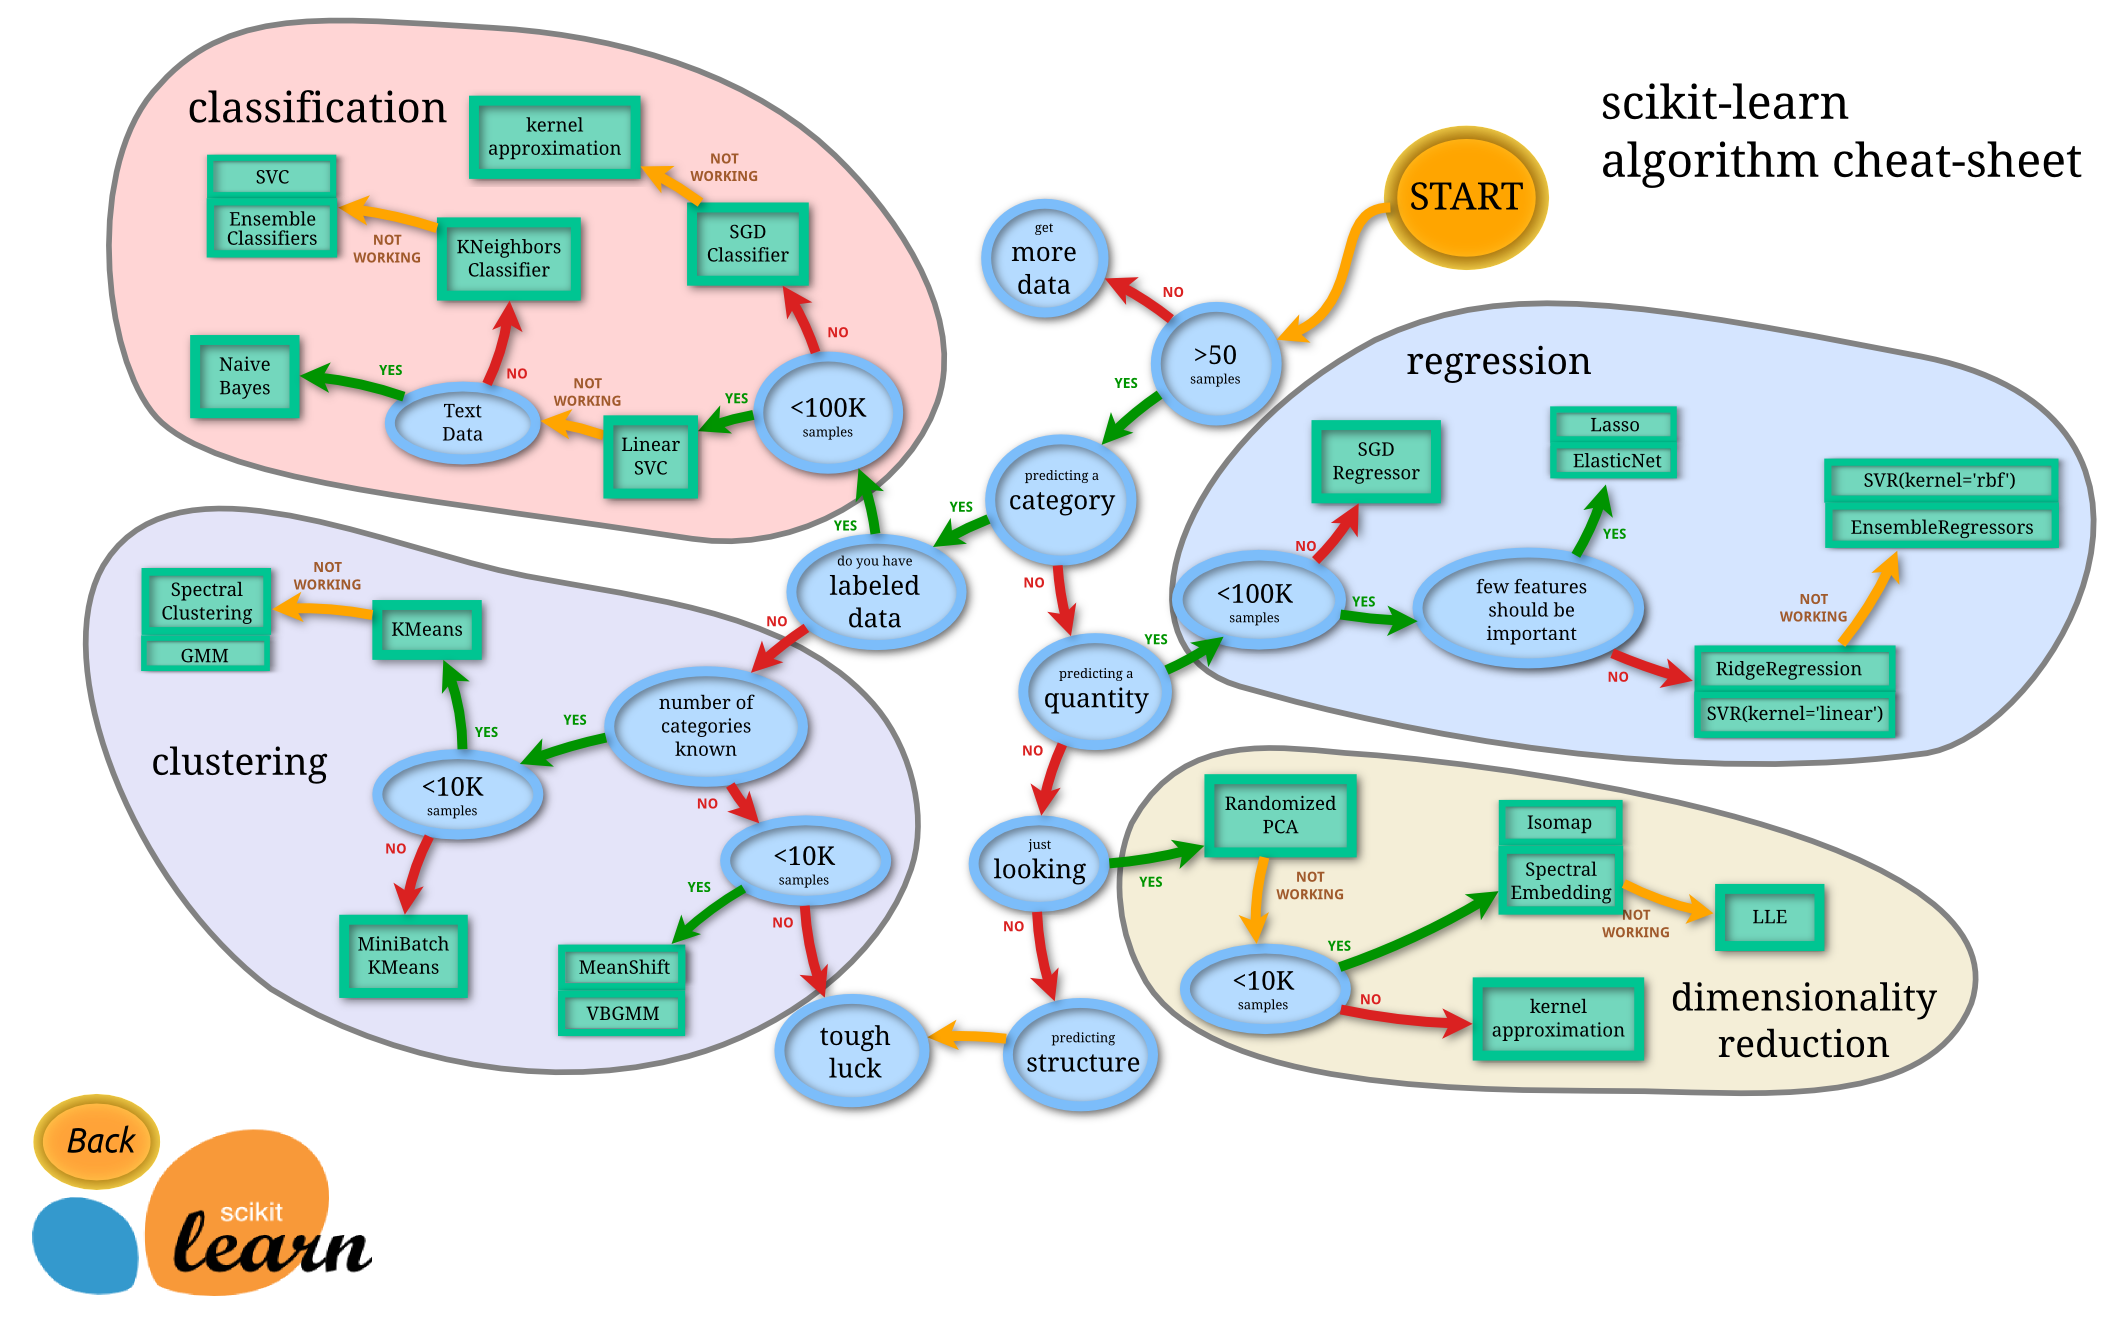
\includegraphics[width=\linewidth]{ml_map.png}
		\caption{Grand catalogue de méthodes de ML}
	\end{figure}
	\end{frame}

\subsection{Types de Machine Learning - Quiz}
	\begin{frame}
	\frametitle{Quiz: Classification ou Regression?}
\begin{itemize}
	\item[1]  Vous avez un large inventaire d'articles identiques. Vous voulez prédire
	combien de ces articles se vendront au cours des 3 prochains mois.
	\item[2]  Vous devez examiner les comptes de vos clients et décider pour chacun d’entre eux s'ils ont été piratés ou compromis. 
	\item[3] Prédiction du churn d'une entreprise
	\item[4] Prédire si un prospect deviendra client
	\item[5] Prédire le chiffre d'affaire d'une entreprise dans 10 ans
\end{itemize}	
\end{frame}		
	
\begin{frame}
	\frametitle{Quiz }
	
	\begin{center}
		\textbf{Given a case study: pricing apartments based on a real estate website.}
	\end{center}
	
	\vspace{0.5cm}
	
	\begin{itemize}
		\item House descriptions with their price
		\item Predicting house prices from their description
		\item Use case: finding houses that are cheap compared to market value
	\end{itemize}
	
\end{frame}

\begin{frame}
	\frametitle{Question 1}
	
	\textbf{What kind of problem is it?}
	
	\begin{enumerate}
		\item[a)] A supervised problem
		\item[b)] An unsupervised problem
		\item[c)] A classification problem
		\item[d)] A regression problem
	\end{enumerate}
	
	\vspace{0.5cm}
	
	\textbf{Select all answers that apply}
	
\end{frame}

\begin{frame}
	\frametitle{Question 2}
	
	\textbf{What are the features?}
	
	\begin{enumerate}
		\item[a)] The number of rooms might be a feature
		\item[b)] The post code of the house might be a feature
		\item[c)] The price of the house might be a feature
	\end{enumerate}
	
	\vspace{0.5cm}
	
	\textbf{Select all answers that apply}
	
\end{frame}

\begin{frame}
	\frametitle{Question 3}
	
	\textbf{What is the target variable?}
	
	\begin{enumerate}
		\item[a)] The full text description is the target
		\item[b)] The price of the house is the target
		\item[c)] Only house descriptions with no price mentioned are the target
	\end{enumerate}
	
	\vspace{0.5cm}
	
	\textbf{Select a single answer}
	
\end{frame}

\begin{frame}
	\frametitle{Question 4}
	
	\textbf{What is a record (a sample, instance)?} (observation)
	
	\begin{enumerate}
		\item[a)] Each house description is a record
		\item[b)] Each house price is a record
		\item[c)] Each kind of description (e.g., house size) is a record
	\end{enumerate}
	
	\vspace{0.5cm}
	
	\textbf{Select a single answer}
	
\end{frame}
	

	
	\begin{frame}{Apprentissage non-supervisé (clustering)}
			\begin{columns}
				\begin{column}{0.5\textwidth}
					\centering
					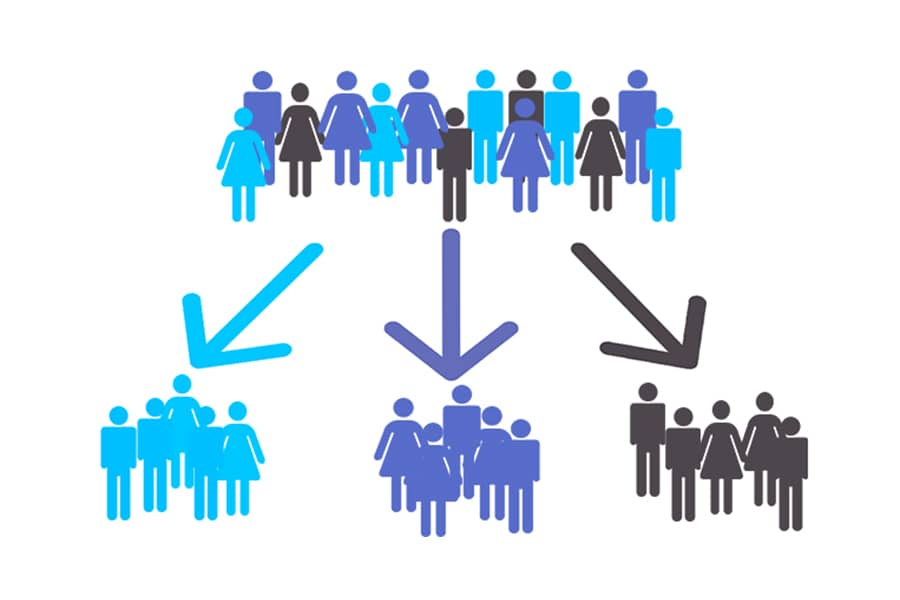
\includegraphics[width=\textwidth]{segmentation.jpg}
					\par
				$3$ Clusters
				\end{column}
				
				\begin{column}{0.5\textwidth}
					\centering
					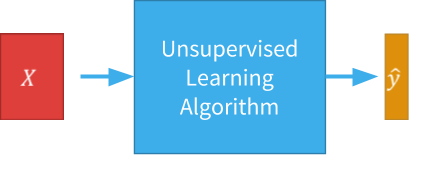
\includegraphics[width=\textwidth]{Machine-Learning-9.png}
					\par
					Principe du clustering
				\end{column}
			\end{columns}
	\end{frame}
	% Slide 8: Conception conceptuelle
		\begin{frame}{Reduction de la dimension}
		\centering
		\begin{figure}[h]
			
\includegraphics[width=0.85\linewidth]{Net.png}
			\caption{Recommendation}
		\end{figure}
	\end{frame}



\begin{frame}{Réduction de la Dimensionnalité}
	\begin{itemize}
		\item Technique utilisée pour réduire le nombre de features d'un dataset.
		\item Objectifs de la réduction de la dimensionnalité :
		\begin{itemize}
			\item Réduire la complexité du modèle et le temps de calcul.
			\item Éliminer les redondances et le bruit dans les données.
			\item Visualiser les données dans un espace de dimension inférieure.
		\end{itemize}
		\item Méthodes courantes de réduction de la dimensionnalité :
		\begin{itemize}
			\item Analyse en composantes principales (PCA) : transforme les variables d'origine en un nouvel ensemble de variables non corrélées appelées CP.
			\item Sélection de caractéristiques : sélectionne un sous-ensemble de caractéristiques les plus informatives.
			\item Manifold Learning : trouve des représentations non linéaires des données dans un espace de dimension inférieure.
		\end{itemize}
	\end{itemize}
\end{frame}
	% Slide 9: Conclusion
	\subsection{Eviter les pièges en ML}
\begin{frame}{Travailler avec les données et éviter les pièges}
	\framesubtitle{Collecte et préparation des données}
	\begin{enumerate}
		\item Collecte des données de qualité et représentatives
			\begin{itemize}
				\item Déterminez les informations que vous voulez collecter
				\item Définissez la méthode de collecte des données
			\end{itemize}
		\item Exploration des données (Data mining)
			\begin{itemize}
				\item Compréhension du problème (activité, objectif)
				\item Compréhension des données
			\end{itemize}
		\item Nettoyage des données 
			\begin{itemize}
				\item Gestion des erreurs de saisie
				\item  Gestion des doublons
				\item  Gestion des valeurs manquantes et des données aberrantes
			\end{itemize}
		\item Les bonnes pratiques de normalisation et transformation des données
	\end{enumerate}
\end{frame}
	
	% Slide 10: Contac
	
\begin{frame}{Travailler avec les données et éviter les pièges}
	\framesubtitle{Sélection des caractéristiques et modélisation}
	\begin{enumerate}
		\item Feature selection (features pertinentes pour le modèle)
		\item Choix et évaluation des modèles
			\begin{itemize}
				\item Sélection du modèle approprié en fonction du problème et des data
				\item L'utilisation de la validation croisée pour évaluer le modèle
				\item L'interprétation des métriques d'évaluation telles que la précision, le rappel, le F1-score, etc.
			\end{itemize}
		\item Gestion du déséquilibre des classes 
		   \begin{itemize}
		   	\item L'identification et la gestion du déséquilibre des classes dans les problèmes de classification
		    \item 	L'utilisation de techniques de suréchantillonnage, de sous-échantillonnage ou d'ajustement des poids des classes pour traiter ce déséquilibre
		   \end{itemize}
		%Réduction du surajustement (overfitting)
			
	\end{enumerate}
\end{frame}


		\begin{frame}{Travailler avec les données et éviter les pièges}
			%\framesubtitle{Surajustement  d'un modèle (overfitting) et under-fitting}
			
	\centering
	\begin{figure}[h]
		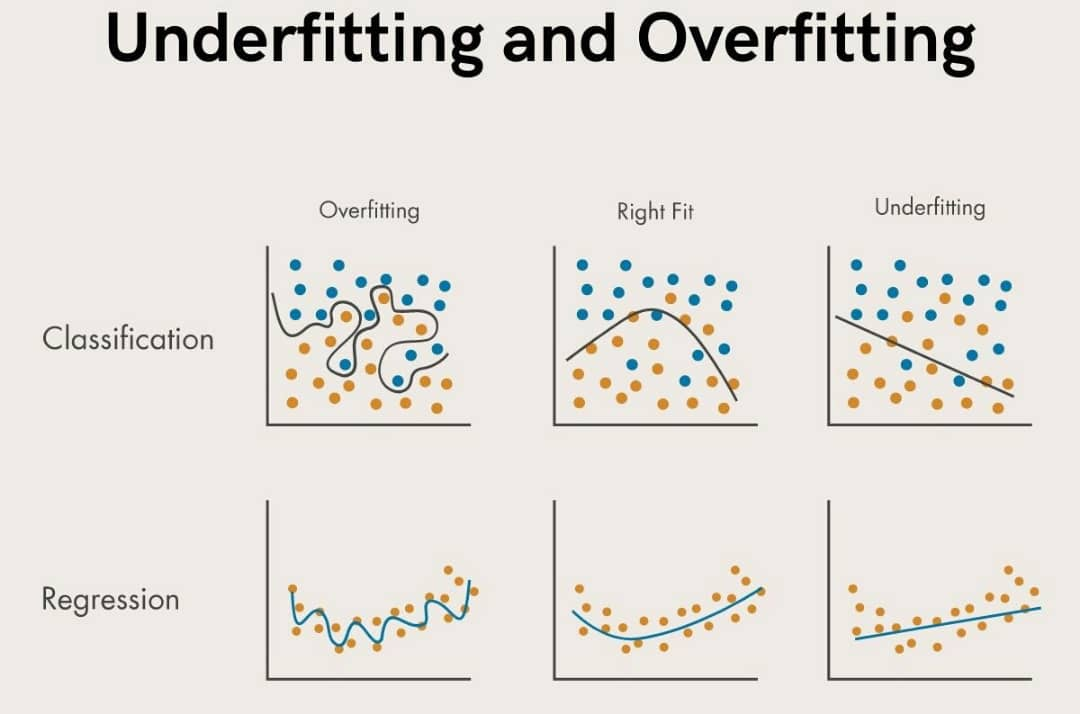
\includegraphics[width=0.75\linewidth]{OverUnderFit.jpeg}
		%\caption{Recommendation}
	\end{figure}
\textbf{	Réduction de l'overfitting }
\begin{itemize}
	\item La compréhension de l'overfitting et ses conséquences
	\item L'utilisation de techniques telles que la régularisation, la validation croisée, le bagging, le boosting, etc.
\end{itemize}
\end{frame}



% Jour 2
\subsection{Quelques modèles de ML}
\begin{frame}{Quelques modèles de Machine Learning}
	\begin{center}
		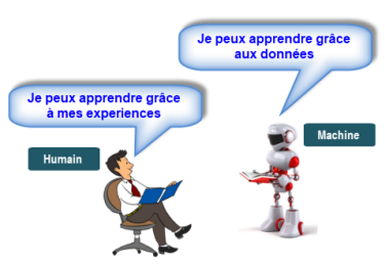
\includegraphics[scale=0.8]{machineLearning.png}
	\end{center}
\end{frame}

\begin{comment}
	\begin{frame}
	\frametitle{Sélection de l'algorithme approprié}
	\begin{itemize}
		\item Importance de choisir le bon algorithme en fonction du problème et des données
		\item Considérations sur la capacité de généralisation, la complexité et l'interprétabilité des modèles
	\end{itemize}
\end{frame}
\end{comment}


\begin{frame}{Modèles de Régression}
	
	\textbf{Régression Linéaire}
	
	\vspace{0.5cm}
	
	Modélisation: relation entre les variables explicatives et la variable cible

	\[
	y = \beta_0 + \beta_1x_1 + \beta_2x_2 + \ldots + \beta_nx_n + \epsilon
	\]
	
	\begin{itemize}
		\item $y$ : Variable dépendante à prédire
		\item $x_1, x_2, \ldots, x_n$ : Variables indépendantes (caractéristiques)
		\item $\beta_0, \beta_1, \beta_2, \ldots, \beta_n$ : Coefficients de régression à estimer
		\item $\epsilon$ : Terme d'erreur aléatoire
	\end{itemize}
	
	\vspace{0.5cm}
	
	\textbf{Régression Logistique}
	\[
	P(y=1) = \frac{1}{1 + e^{-(\beta_0 + \beta_1x_1 + \beta_2x_2 + \ldots + \beta_nx_n)}}
	\]
	
	\begin{itemize}
		\item $P(y=1)$ : Probabilité que la variable dépendante $y$ prenne la valeur 1
		\item $x_1, x_2, \ldots, x_n$ : features.
	\end{itemize}
	
\end{frame}


\begin{frame}{Arbre de Décision}
	\begin{itemize}
		\item Modèle d'apprentissage automatique non linéaire et non paramétrique
		\item Représente une série de décisions basées sur les features
		\item Utilisé pour la classification et la régression
	\end{itemize}
	
	\begin{center}
		\begin{figure}
	%	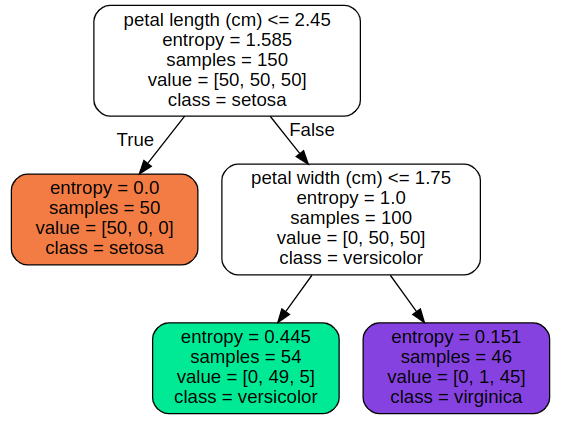
\includegraphics[width=0.6\textwidth]{iris.png}
		    \begin{minipage}[t]{0.45\linewidth}
			\centering
			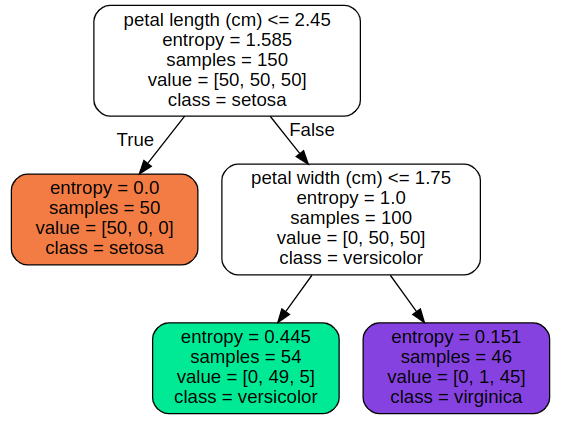
\includegraphics[width=\linewidth]{iris.png}
			\caption{Classification tree}
		\end{minipage}
		\hfill
		\begin{minipage}[t]{0.45\linewidth}
			\centering
			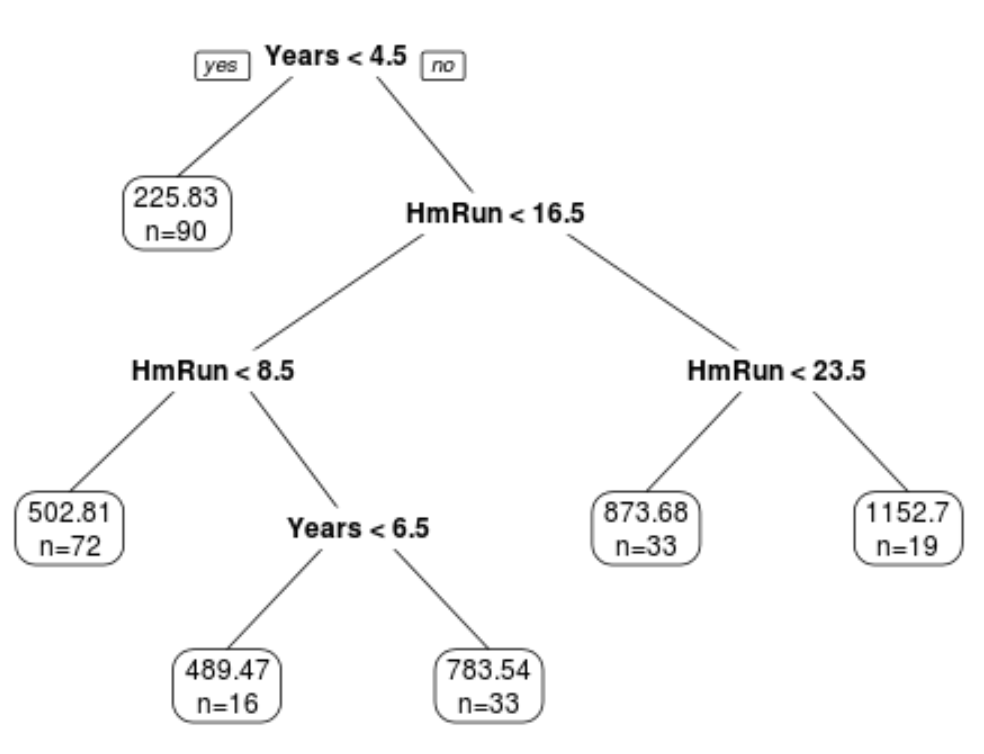
\includegraphics[width=\linewidth]{Rtree3.png}
			\caption{Regression tree}
		\end{minipage}
\end{figure}
\end{center}
\end{frame}

\begin{frame}{Machines à Vecteurs de Support (SVM)}
	\begin{itemize}
		\item Modèle d'apprentissage automatique supervisé
		\item Utilisé pour la classification et la régression
		\item Trouve un hyperplan optimal qui sépare les données de différentes classes ou estime une fonction pour la régression
		\item Maximise la marge entre les données et l'hyperplan pour une meilleure généralisation
	\end{itemize}
	
	%\begin{center}
	%	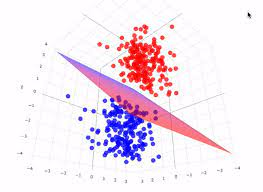
\includegraphics[width=0.6\textwidth]{csvm.jpeg}
	%\end{center}
	  \begin{figure}
	  	 \begin{minipage}[t]{0.45\linewidth}
		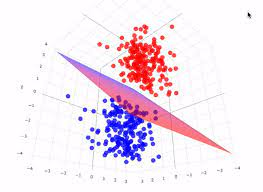
\includegraphics[width=\linewidth]{csvm.jpeg}
		\caption{Support Vector Classifier}
	\end{minipage}
	\hfill
	\begin{minipage}[t]{0.45\linewidth}
		\centering
		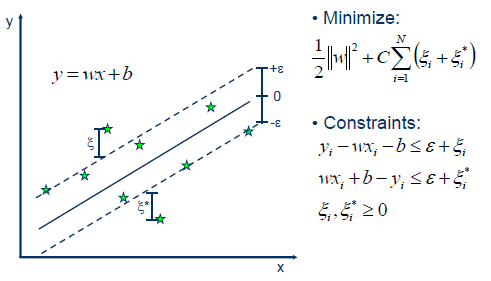
\includegraphics[width=\linewidth]{SVR_2.png}
		\caption{Support Vector Regressor}
	\end{minipage}
	  \end{figure}
\end{frame}


\begin{frame}{Forêt Aléatoire (Random Forest)}
	\begin{itemize}
	%	\item Méthode d'apprentissage automatique utilisée pour la classification et la régression
		\item Basée sur l'ensemble de plusieurs arbres de décision
		\item Chaque arbre est construit sur un sous-ensemble aléatoire des données d'entraînement et des caractéristiques
		\item Les prédictions finales sont obtenues en agrégeant les prédictions de chaque arbre (majorité pour la classification, moyenne pour la régression)
	\end{itemize}
	
	\begin{center}
		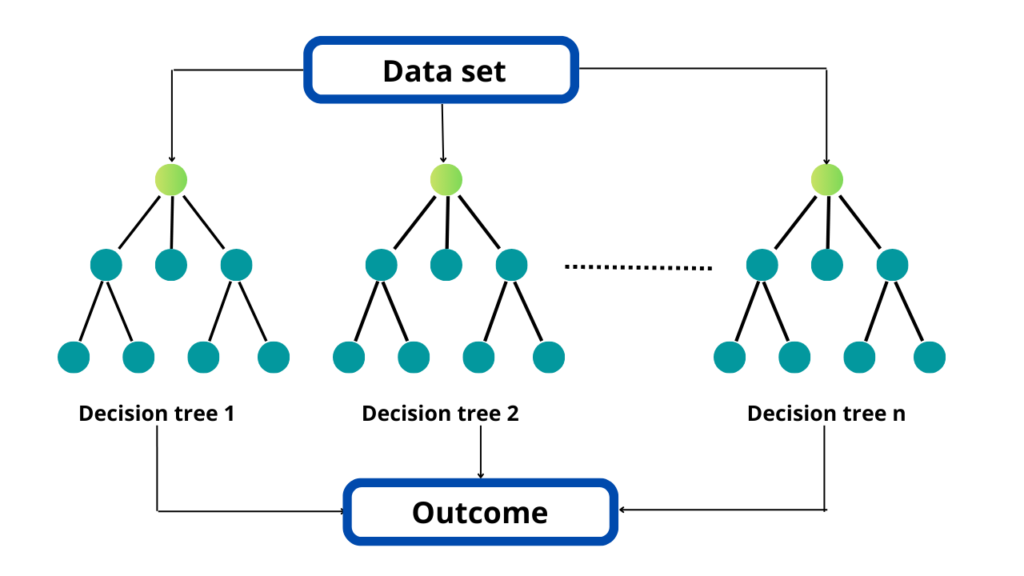
\includegraphics[width=0.6\textwidth]{destree.png}
	\end{center}
\end{frame}

\begin{frame}{Boosting}
	\begin{itemize}
		\item Technique de ML utilisée pour améliorer la performance des modèles
		\item Combinaison \color{blue} séquentielle \color{black}
		de modèles faibles pour former un fort
		\item Chaque modèle faible est entraîné à se concentrer sur les échantillons mal classés par les modèles précédents
		\item Les prédictions finales sont obtenues en agrégeant les prédictions de chaque modèle faible (pondération selon leur performance)
	\end{itemize}
	
	\begin{center}
		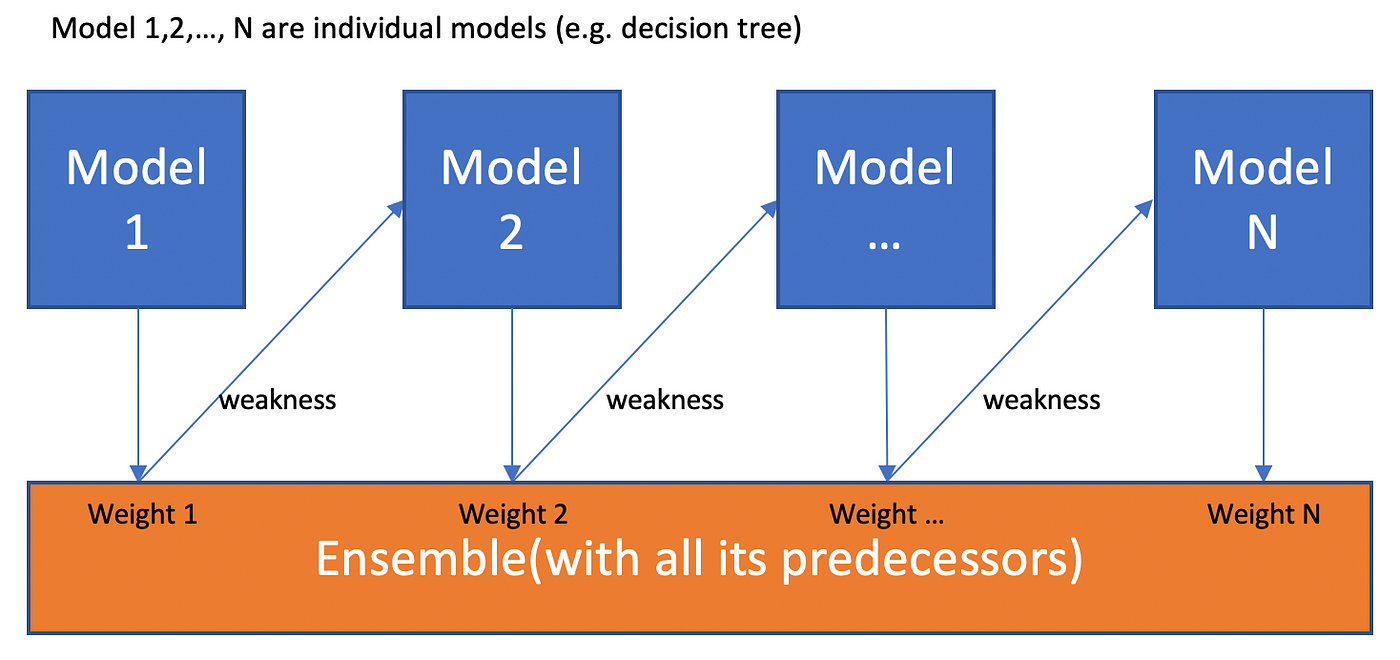
\includegraphics[width=0.6\textwidth]{boosting.png}
	\end{center}
\end{frame}



\begin{frame}{Boosting vs Bagging}
	\begin{columns}
		\begin{column}{0.5\textwidth}
			\textbf{Boosting}
			\begin{itemize}
				\item Combinaison séquentielle de modèles faibles
				\item Chaque modèle se concentre sur les échantillons mal classés par les modèles précédents
				\item Biais réduit, forte capacité de généralisation
				\item Sensible aux données d'entraînement bruitées ou aberrantes
			\end{itemize}
		\end{column}
		\begin{column}{0.5\textwidth}
			\textbf{Bagging}
			\begin{itemize}
				\item Combinaison parallèle de modèles indépendants
				\item Chaque modèle est entraîné sur un sous-ensemble aléatoire des données d'entraînement
				\item Réduction de la variance, faible risque de surajustement
				\item Moins sensible aux données bruitées ou aberrantes
			\end{itemize}
		\end{column}
	\end{columns}
\end{frame}


\begin{frame}{Évaluation des modèles}
	\begin{itemize}
		\item L'évaluation des modèles est essentielle pour mesurer leur performance et prendre des décisions informées.
		\item Métriques de performance couramment utilisées :
		\begin{itemize}
			\item Précision : mesure la proportion de prédictions positives correctes.
			\item Rappel : mesure la proportion de vrais positifs identifiés.
			\item F-mesure : combine la précision et le rappel en une seule métrique.
			\item Exactitude : mesure la proportion de prédictions correctes dans l'ensemble des données.
			\item Courbe ROC : représente la sensibilité (rappel) en fonction de la spécificité.
		\end{itemize}
		\item Techniques d'évaluation :
		\begin{itemize}
			\item Validation croisée : divise les données en ensembles d'entraînement et de test pour évaluer la performance.
			\item Holdout : divise les données en un ensemble d'entraînement et un ensemble de test.
			\item Bootstrap : utilise des échantillons bootstrap pour estimer la performance du modèle.
		\end{itemize}
	\end{itemize}
\end{frame}

\begin{comment}
	\begin{frame}
	\frametitle{Mesure du succès et ajustement des hyperparamètres}
	\begin{itemize}
		\item Choix des métriques appropriées pour mesurer le succès du modèle en fonction du problème
		\item Optimisation des hyperparamètres pour améliorer la performance du modèle
		\item Utilisation de méthodes comme la recherche en grille et l'optimisation bayésienne
	\end{itemize}
\end{frame}
\end{comment}




\begin{frame}{Conclusion}
	\begin{itemize}
		\item Le Machine Learning est une approche d'intelligence artificielle qui permet aux ordinateurs d'apprendre à partir des données sans être explicitement programmés.
		\item Le processus de Machine Learning comprend :
		\begin{enumerate}
			\item Collecte des données d'entraînement.
			\item Sélection du modèle approprié.
			\item Entraînement du modèle sur les données d'entraînement.
			\item Évaluation de la performance du modèle sur des données de test.
			\item Utilisation du modèle entraîné pour faire des prédictions sur de nouvelles données.
		\end{enumerate}
		\item Les algorithmes d'apprentissage automatique peuvent être supervisés ou non supervisés.
		\item L'objectif du Machine Learning est de généraliser à partir des données d'entraînement afin de faire des prédictions précises sur de nouvelles données non vues auparavant.
	\end{itemize}
\end{frame}



\section{Artificial Intelligence and Machine Learning 2}

{
\setbeamertemplate{background}{
\includegraphics[width=\paperwidth,height=\paperheight]{ia_ml.jpg}}	
\begin{frame}{Artificial Intelligence and Machine Learning 2}
	%\centering
%	
\includegraphics[width=\linewidth]{ia_ml.jpg}
\end{frame}

}





\begin{frame}
	\frametitle{Plan de présentation}
	\begin{itemize}
		\item Introduction
		\begin{itemize}
			\item Contexte et objectifs
		\end{itemize}
		\item XAI et IML : Explicabilité dans l'IA et le ML
		\begin{itemize}
			\item Comprendre XAI et IML
			\item Difficultés liées à l'isolation de la contribution d'une variable
			\item Modèle de boîte noire 101
		\end{itemize}
		\item KNIME pour XAI et IML
		\begin{itemize}
			\item Présentation de KNIME
			\item Utilisation de KNIME pour l'explicabilité et l'interprétabilité
			\item Exemples d'utilisation de KNIME dans XAI et IML
		\end{itemize}
		\item Techniques de XAI : Explications globales
		\begin{itemize}
			\item Obtenir des explications globales
			\item Techniques : importance des variables, arbres de décision, règles d'association, etc.
			\item Avantages et limitations des techniques d'explication globale
		\end{itemize}
		% Ajoutez les autres sections de la même manière
	\end{itemize}
\end{frame}

	
\subsection{Introduction}	
\begin{frame}{Vue d'ensemble des concepts clés}
	\begin{itemize}
		\item Qu'est-ce que l'Explainable AI (XAI) et l'Interprétabilité en ML (IML)?
		\item Les défis de l'isolement de la contribution d'une variable
		\item Modèle de boîte noire 101 : Comprendre les modèles opaques
		\item KNIME pour XAI et IML : Une introduction à l'outil
		\item Techniques d'Explainable AI (XAI) : explications globales, explications locales
		\item Techniques d'Interprétabilité en Machine Learning (IML) : visualisation, importance des variables, etc.
		\item Conception expérimentale et contrôles statistiques : l'importance de la planification et des comparaisons de modèles
		\item Conditionnel Probabilité et théorème de Bayes : Mise à jour des probabilités
		\item Prédiction et preuve avec les statistiques bayésiennes : Introduction aux statistiques bayésiennes
		\item Modélisation causale : Modélisation d'équations structurelles (SEM), réseaux bayésiens
		\item Importance d'une valeur p pour le test d'hypothèse : Définition, différence entre corrélation et causalité, démonstration de la causalité
		\item Détection de la multicolinéarité et stratégies associées
		\item Induction, déduction, falsification et contrefactuel : Importance dans l'évaluation du modèle
		\item Utilité décroissante des valeurs p avec un nombre croissant de paramètres de modèle : Explication
		\item Évaluation des performances du modèle dans l'exploration de données : Objectifs et philosophie contradictoires des statistiques et de l'exploration de données
		\item Apprentissage par renforcement : Introduction, algorithmes et méthodes associées
	\end{itemize}
\end{frame}
	
\subsection{XAI et IML : Explicabilité dans l'IA et le ML}	
\begin{frame}{Explainable AI (XAI) et Interprétabilité en ML (IML)}
	\begin{itemize}
		\item L'Explainable AI (XAI) et l'Interprétabilité en ML (IML) visent à rendre les modèles de ML plus compréhensibles et expliquables pour les humains.
		\item L'IML : compréhension des décisions prises par les modèles, alors que le XAI vise à expliquer le fonctionnement interne des modèles.
		\item L'importance de l'IML et du XAI :
		\begin{itemize}
			\item Gagner la confiance des utilisateurs et des parties prenantes.
			\item Détecter les biais et les erreurs de modélisation.
			\item Se conformer aux réglementations et aux normes éthiques.
			\item Faciliter la résolution des problèmes lorsque les modèles produisent des résultats inattendus ou incorrects.
		\end{itemize}
		\item Techniques d'IML et de XAI :
		\begin{itemize}
			\item Visualisation des caractéristiques importantes.
			\item Interprétation des poids des modèles linéaires.
			\item Méthodes d'interprétabilité spécifiques à certains algorithmes(des tree).
			\item Utilisation de modèles explicatifs, tels que les réseaux de neurones à propagation avant avec des couches interprétables.
		\end{itemize}
	\end{itemize}
\end{frame}
	
\begin{frame}{Les défis de l'isolement de la contribution d'une variable}
	\begin{itemize}
		\item Les défis courants de l'isolation de la contribution d'une va en ML :
		\begin{itemize}
			\item Corrélations 
			%: les variables sont souvent corrélées entre elles, ce qui rend difficile de déterminer la contribution spécifique d'une variable sans tenir compte des autres.
			\item Interactions 
			%: les variables peuvent interagir de manière complexe, ce qui rend difficile d'attribuer une contribution individuelle à chaque va.
			\item Non-linéarité : les relations entre les variables et la variable cible peuvent être non linéaires, ce qui complique l'isolement des contributions individuelles.
			\item Multicollinéarité
			% : lorsque plusieurs variables sont fortement corrélées, il peut être difficile de distinguer leur contribution individuelle.
		\end{itemize}
		\item Méthodes pour aborder ces défis :
		\begin{itemize}
			\item Analyse de sensibilité : évaluer l'impact d'une variable en la modifiant de manière contrôlée tout en maintenant les autres variables constantes.
			\item Décomposition de la variance : attribuer une part de la variance expliquée à chaque variable.
			\item Méthodes d'importance de variable : estimer l'importance relative des variables en utilisant des techniques telles que les arbres de décision ou les coefficients de régression.
		\end{itemize}
	\end{itemize}
\end{frame}


\begin{frame}{Modèle de boîte noire 101 : Modèles opaques}
\begin{center}
	\begin{figure}
			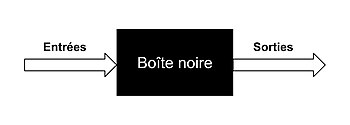
\includegraphics[width=0.6\linewidth]{350px-Schéma_d'une_boîte_noire.jpg}
	\end{figure}
\end{center}
	\begin{itemize}
		\item Modèles d'IA dont les mécanismes internes sont difficiles à interpréter.
		\item Modèles très performants en termes de prédiction, mais souvent difficile à comprendre.
		\item Les modèles opaques (DNN ou SVM) peuvent avoir des millions de paramètres et des architectures complexes.
		\item L'opacité de ces modèles pose des défis en termes de transparence, d'éthique et d'acceptabilité sociale de l'IA.
		\item Malgré leur complexité, XAI et IML tentent de les comprendre.
	\end{itemize}

\end{frame}



\begin{frame}{KNIME pour XAI et IML : Une introduction à l'outil}
	\begin{itemize}
		\item KNIME est une plateforme open-source d'analyse des données et de construction de workflows.
		\item Il offre une interface intuitive et conviviale pour créer, exécuter et partager des workflows d'analyse de données.
		\item KNIME propose également une large gamme de modules et d'extensions pour XAI et l'IML.
		\item Avec KNIME, vous pouvez appliquer des techniques d'XAI pour comprendre comment les modèles prennent des décisions et les expliquer de manière compréhensible.
		\item Vous pouvez également utiliser des modules d'IML pour visualiser et interpréter les résultats de vos modèles, tels que l'importance des variables, les poids des coefficients, etc.
		\item KNIME offre une flexibilité et une extensibilité importantes, vous permettant d'adapter facilement vos workflows aux besoins spécifiques de votre projet.
	\end{itemize}
\end{frame}













\begin{frame}{Techniques XAI : explications globales, explications locales}
	\begin{itemize}
		\item Les techniques XAI sont des méthodes utilisées pour expliquer les décisions prises par les modèles d'IA.
		\item Les explications globales fournissent une vue d'ensemble du modèle et de ses principaux facteurs de décision, permettant de comprendre le comportement général du modèle.
		\item Les techniques d'explication globale incluent des méthodes telles que les diagrammes d'importance de variables, les graphiques de dépendance partielle et les cartes de chaleur.
	
		\item Les explications locales se concentrent sur une prédiction spécifique et fournissent une explication détaillée de la contribution de chaque variable à cette prédiction.
		\item Les techniques d'explication locale incluent des méthodes telles que les perturbations de variable, les méthodes de désensibilisation et les arbres de décision locaux.
		\item Compréhension fine des facteurs qui ont conduit à une prédiction spécifique, ce qui peut aider à détecter les biais, les erreurs ou les cas extrêmes.

	\end{itemize}
\end{frame}

\begin{frame}{Techniques IML : visualisation, importance des variables}
	\begin{itemize}
		\item La visualisation permet d'explorer et de comprendre les relations entre les variables et les résultats du modèle.
		\item Les graphiques, les diagrammes et les cartes peuvent être utilisés pour représenter les données de manière intuitive et faciliter l'interprétation.
		\item L'importance des variables est une autre technique d'IML qui permet d'identifier les variables qui ont le plus d'influence sur les prédictions du modèle.
		\item Les méthodes d'importance des variables incluent l'analyse de sensibilité, le calcul des coefficients ou des poids des variables et les techniques d'élagage.

		\item En combinant la visualisation des données, l'importance des variables et d'autres techniques d'IML, on peut obtenir une compréhension approfondie du modèle de ML et de ses mécanismes de décision.

	\end{itemize}
\end{frame}




\begin{frame}{Conception expérimentale et contrôles statistiques}
	\begin{itemize}

		\item Planification : définition claire des objectifs de l'expérience, choix des features à mesurer, échantillonnage.
		\item Les comparaisons de modèles
		\item Des techniques statistiques telles que les tests d'hypothèse, l'ANOVA et les tests de comparaison multiple 
		\item Il est également important de prendre en compte les biais potentiels
		\item Une planification et des contrôles appropriés permettent de minimiser les erreurs expérimentales, d'obtenir des résultats précis et de fournir des informations utiles pour prendre des décisions éclairées en matière de modélisation.
		\item En fin de compte, la conception expérimentale et les contrôles statistiques renforcent la validité et la crédibilité des résultats obtenus à partir des modèles d'IA.
	\end{itemize}
\end{frame}




\begin{frame}{Probabilité Conditionnelle et théorème de Bayes}
	\begin{itemize}
		
		\item Elle est notée $P(A|B)$ et se calcule suivant la relation $$P(A|B) = \frac{P(A\cap B)}{P(B)}$$
		\item Le théorème de Bayes permet de mettre à jour les probabilités conditionnelles lorsque de nouvelles informations sont disponibles.
		\item La formule de Bayes est donnée par  $$P(A|B) = \frac{P(B|A) * P(A)}{P(B)} $$.
		\item Le théorème de Bayes est largement utilisé dans les domaines de la statistique, du ML et de l'IA pour la prise de décision.
		\item Il permet de mettre à jour les probabilités a priori en fonction des nouvelles observations, ce qui permet d'obtenir des estimations plus précises et fiables.

%		\item En utilisant le théorème de Bayes, on peut incorporer de nouvelles informations dans un modèle probabiliste et obtenir une estimation plus précise des probabilités conditionnelles.
	\end{itemize}
\end{frame}



\begin{frame}{Introduction aux statistiques bayésiennes}
	\begin{itemize}
%		\item Les statistiques bayésiennes utilisent la théorie des probabilités bayésiennes pour modéliser et analyser les données.
		\item Contrairement aux statistiques fréquentistes, les statistiques bayésiennes considèrent les paramètres comme des v.a avec des dp.
		\item L'analyse bayésienne commence par une distribution a priori pour les paramètres, puis met à jour cette distribution en utilisant le théorème de Bayes pour obtenir une distribution a posteriori.
		\item La distribution a posteriori est utilisée pour effectuer des prédictions et des estimations, en tenant compte de l'incertitude associée aux résultats.
		\item Les statistiques bayésiennes permettent également de comparer des modèles en utilisant des facteurs de Bayes, qui intègrent la vraisemblance des données et la complexité des modèles.
		\item Les statistiques bayésiennes offrent une approche cohérente et intuitive pour la prise de décision en intégrant les connaissances préalables et les données observées.
		\item Cependant, l'analyse bayésienne peut nécessiter des techniques d'inférence approximative, telles que les chaînes de Markov Monte Carlo (MCMC).
	\end{itemize}
\end{frame}



\begin{frame}{Modélisation causale : Modélisation d'équations structurelles (SEM), réseaux bayésiens}
	\begin{itemize}
		\item La modélisation causale vise à comprendre les relations de cause à effet entre les variables dans un système.
		\item Les équations structurelles (SEM) et les réseaux bayésiens sont deux approches couramment utilisées en modélisation causale.
		\item Les SEM sont des modèles qui représentent les relations causales entre les variables à l'aide d'équations mathématiques.
		\item Les SEM permettent de tester des hypothèses causales.
		\item Les réseaux bayésiens, quant à eux, utilisent des graphes probabilistes pour représenter les relations causales entre les variables.
		\item Les réseaux bayésiens intègrent également des connaissances a priori et des distributions de probabilité pour quantifier l'incertitude dans la modélisation causale.
		\item Ces approches permettent de faire des prédictions causales, d'identifier les variables clés et de tester les hypothèses causales.
	\end{itemize}
\end{frame}





	
	
	\begin{frame}{Statistiques et tests d'hypothèse}
		\begin{itemize}
			\item La $p-$value est utilisée pour évaluer les preuves contre l'hypothèse $H_0$.
			\item Une $p-$value faible indique une preuve solide contre $H_0$.
			\item La $p-$value seule ne fournit pas d'informations sur la taille de l'effet ou la signification pratique des résultats.
			\item L'interprétation doit tenir compte de la $p-$value et de l'importance clinique ou scientifique des résultats.
		\end{itemize}
		
		\vfill
		
		\begin{itemize}
			\item La corrélation mesure la relation statistique entre deux variables.
			\item La causalité nécessite des preuves supplémentaires, comme des expérimentations contrôlées.
			\item Les études observationnelles fournissent des indications de relation causale, mais ne prouvent pas définitivement l'existence de la causalité.
		\end{itemize}
		
%		\vfill
		
		%\begin{itemize}
		%	\item La démonstration de la causalité nécessite souvent des expériences contrôlées.
		%	\item Les groupes d'expérimentation et de contrôle permettent de comparer les résultats.
		%	\item Dans certains domaines, il peut être difficile de réaliser des expériences contrôlées.
	%	\end{itemize}
	\end{frame}
	

\begin{frame}{Détection de la multicolinéarité et stratégies associées}
	\textbf{Détection de la multicolinéarité :}
	\begin{itemize}
		\item Calcul des coefficients de corrélation.
		\item Variance inflation factor (VIF).
		\item Analyse des valeurs propres.
	\end{itemize}
	
	\vfill
	
	\textbf{Stratégies pour traiter la multicolinéarité :}
	\begin{itemize}
		\item Supprimer les variables fortement corrélées.
		\item Combinaison de variables corrélées.
		\item Utilisation de techniques de régularisation (régression ridge, régression lasso).
	\end{itemize}
	
	\vfill
	
	\textbf{Remarque :} Les approches de détection et de gestion de la multicolinéarité doivent être adaptées au contexte spécifique de l'analyse et aux objectifs de modélisation.
\end{frame}


\begin{frame}{Induction, déduction, falsification et contrefactuel : Importance dans l'évaluation du modèle}
	\begin{itemize}
		\item \textbf{Induction :} Permet de généraliser à partir des observations spécifiques et de tirer des conclusions sur des situations non observées.
		\item \textbf{Déduction :} Utilisation de règles logiques pour déduire des conséquences spécifiques à partir de propositions générales. Peut aider à tester les prédictions d'un modèle.
		\item \textbf{Falsification :} Processus de recherche d'observations ou de tests qui pourraient réfuter ou invalider un modèle. Contribue à la rigueur et à la fiabilité d'un modèle.
		\item \textbf{Contrefactuel :} Étudie les effets hypothétiques d'un changement dans les conditions ou les variables. Permet d'évaluer l'impact causal et de comparer différentes situations.
	\end{itemize}
	
	\vfill
	
	L'utilisation appropriée de ces concepts contribue à une évaluation rigoureuse et solide des modèles, en tenant compte à la fois des preuves empiriques et des raisonnements logiques.
\end{frame}


\begin{frame}{Utilité décroissante des valeurs p avec un nombre croissant de paramètres de modèle : Explication}
	\begin{itemize}
		\item Lorsque le nombre de paramètres d'un modèle statistique augmente, les valeurs p associées à ces paramètres ont tendance à diminuer.
		\item Les valeurs p mesurent la significativité statistique d'un paramètre en évaluant la probabilité d'obtenir des résultats aussi extrêmes que ceux observés, sous l'hypothèse nulle.
		\item Cependant, avec un nombre croissant de paramètres, il y a une augmentation du nombre de tests statistiques effectués, ce qui peut conduire à une augmentation des chances de trouver des associations significatives par pur hasard.
		\item Ce phénomène est connu sous le nom d'utilité décroissante des valeurs p et est causé par le problème de multiplicité des tests.
		\item Plus il y a de paramètres à tester, plus il est probable d'obtenir des associations significatives par simple hasard, même en l'absence de relations réelles entre les variables.
		\item Cela souligne l'importance de prendre en compte le contexte scientifique, la taille de l'échantillon et la pertinence des relations dans l'interprétation des valeurs p.
		\item Des méthodes correctives, telles que l'ajustement de Bonferroni ou les procédures de contrôle de la fausse découverte, peuvent être utilisées pour tenir compte du problème de multiplicité des tests.
		\item Il est essentiel de considérer ces aspects lors de l'évaluation et de l'interprétation des résultats statistiques.
	\end{itemize}
\end{frame}


\begin{frame}{Évaluation des performances du modèle dans l'EDA}
	\begin{itemize}
		\item L'évaluation des performances du modèle est une étape essentielle dans l'exploration de données, visant à évaluer la qualité et l'adéquation d'un modèle pour représenter les données.
		\item Les statistiques et l'exploration de données ont des objectifs et des philosophies souvent contradictoires dans cette évaluation.
		\item Les statistiques traditionnelles se concentrent sur la précision et la validité des modèles, en utilisant des méthodes rigoureuses basées sur des hypothèses et des tests statistiques.
		\item Les statistiques mettent l'accent sur la généralisation des résultats, la réduction de l'incertitude et la déduction causale.
		\item En revanche, l'exploration de données se concentre sur la découverte de nouvelles connaissances, l'identification de modèles intéressants et la génération d'hypothèses.
		\item L'exploration de données privilégie l'exploration des données brutes, l'utilisation de techniques non paramétriques et l'incorporation de l'expertise humaine.
		\item L'objectif de l'exploration de données est de fournir des informations exploitables et de soutenir la prise de décision, même si cela peut impliquer une certaine incertitude et une moindre généralisation.
		\item Il est important de reconnaître que les statistiques et l'exploration de données sont complémentaires et peuvent être utilisées conjointement pour une évaluation plus complète des performances du modèle.
	\end{itemize}
\end{frame}



\begin{frame}
	\frametitle{Conclusion}
	\begin{itemize}
		\item Récapitulatif des concepts clés abordés dans les applications pratiques de l'IA et du Machine Learning
		\item Invitation aux questions et discussions
	\end{itemize}
\end{frame}

\section{Artificial Intelligence and Machine Learning 3}

{
	\setbeamertemplate{background}{\includegraphics[width=\paperwidth,height=\paperheight]{ia_ml.jpg}}
\begin{frame}{Artificial Intelligence and Machine Learning 3}
	%\centering
	%\includegraphics[width=\linewidth]{ia_ml.jpg}
\end{frame}

}




\begin{frame}
	\frametitle{Plan de présentation}
	\begin{itemize}
		\item Examen des défis de l'IA
		\item Application de l'IA étroite à une décision
		\item Définition de deux approches efficaces utilisées face à l'IA
		\item Examen de l'apprentissage supervisé et non supervisé
		\item Explication du harcèlement par l'IA
		\item Identification de trois concepts sur lesquels repose la justice distributive
		\item Qu'est-ce que XAI (IA explicative) ?
		\item Avantages et limites de XAI
		\item Humains par rapport aux ordinateurs
		\item Exemples commerciaux de XAI
		\item Investir dans XAI
		\item Transformateurs en PNL
		\item Formation des transformateurs et leur architecture
		\item Grands modèles de langage
		\item Présentation des arbres de décision
		\item Présentation de l'algorithme C5.0
		\item Présentation des arbres de classification
		\item Présentation des arbres de régression
		\item NPL et transformateurs
		\item BERT et apprentissage par transfert
		\item Architecture de transformateur et BERT
		\item Classification de texte
		% Ajoutez les autres sections de la même manière
	\end{itemize}
\end{frame}


\subsection{Examen des défis de l'IA}
\begin{frame}{Examen des défis de l'IA}
	\begin{columns}[T]
		\begin{column}{0.5\textwidth}
			\begin{itemize}
				\item Manque de transparence des modèles d'IA
				\item Biais et résultats discriminatoires
				\item Problèmes d'éthique et de confidentialité
				\item Impact sur l'emploi
				\item Besoin de big data
				\item Sécurité des systèmes d'IA
			\end{itemize}
		\end{column}
		\begin{column}{0.5\textwidth}
			\includegraphics[width=\textwidth]{AI-ethics.jpg}
		\end{column}
	\end{columns}
\end{frame}

\begin{frame}{Définition de deux approches efficaces utilisées face à l'IA}
	\begin{columns}[T]
		\begin{column}{0.5\textwidth}
			\textbf{Apprentissage supervisé}
			\begin{itemize}
				\item Utilise des données étiquetées
				\item Prédit des résultats pour de nouvelles données
				\item Exemples : classification, prédiction
			\end{itemize}
		\end{column}
		\begin{column}{0.5\textwidth}
			\textbf{Apprentissage non supervisé}
			\begin{itemize}
				\item Utilise des données non étiquetées
				\item Découvre des structures, des modèles ou des relations
				\item Exemples : regroupement, réduction de dimensionnalité
			\end{itemize}
		\end{column}
	\end{columns}
	\vspace{0.5cm}
	\centering
	\includegraphics[width=0.8\textwidth]{approachesdata.png}
\end{frame}

\begin{frame}{Application de l'IA étroite à une décision}
	\begin{itemize}
		\item L'IA étroite ou IA faible, se réfère à des systèmes d'IA conçus pour effectuer des tâches spécifiques avec une grande précision.
		\item Ces systèmes d'IA sont utilisées en reconnaissance d'image,vtraduction automatique, détection de fraude, etc.
		\item L'IA étroite est utilisée dans les systèmes de recommandation personnalisée ou les chatbots de service client.
		\item Les systèmes d'IA étroite utilisent des algorithmes sophistiqués et des techniques de ML.
		\item Limites: incapacité à reproduire pleinement les capacités cognitives humaines (compréhension du contexte, de flexibilité et de raisonnement abstrait).
		%\item Compréhension des domaines dans lesquels l'IA étroite peut être appliquée de manière efficace et les limites de son utilisation afin d'éviter des erreurs ou des résultats inappropriés.
	\end{itemize}
\end{frame}



\begin{frame}{Explication du harcèlement par l'IA}
	\begin{columns}[T]
		\begin{column}{0.6\textwidth}
			\begin{itemize}
				\item Génération de contenu haineux
				\item Ciblage et traque en ligne
				\item Biais et discrimination
			\end{itemize}
		\end{column}
		\begin{column}{0.4\textwidth}
			\includegraphics[width=\textwidth]{harcellement.png}
		\end{column}
	\end{columns}
	
	\vspace{0.5cm}
	
	\begin{itemize}
		\item Les modèles d'IA peuvent être exploités pour générer automatiquement du contenu haineux et offensant.
		\item Les algorithmes d'IA peuvent être utilisés pour cibler et harceler des individus en ligne.
		\item Les biais et préjugés présents dans les données d'entraînement peuvent conduire à une discrimination automatique.
	\end{itemize}
\end{frame}


\begin{frame}{Concepts clés de la justice distributive}
	\textbf{Égalité}
	\begin{itemize}
		\item Principe fondamental de la justice distributive
		\item Répartition équitable des ressources et des avantages
		\item Élimination de la discrimination basée sur des features personnelles
	\end{itemize}
	
	\vspace{0.3cm}
	
	\textbf{Besoins}
	\begin{itemize}
		\item Prise en compte des besoins réels des individus
		\item Attribution des ressources en fonction des besoins urgents ou essentiels
		\item Exemple : priorité d'accès aux soins pour les personnes malades
	\end{itemize}
	
	\vspace{0.3cm}
	
	\textbf{Mérite}
	\begin{itemize}
		\item Distribution des ressources en fonction du mérite ou de la contribution
		\item Récompense des gens pour leur travail, compétences ou contribution
		\item Exemple : rémunération plus élevée pour les compétences spécialisées ou les emplois valorisés
	\end{itemize}
\end{frame}

\subsection{XAI (IA explicative)}
\begin{frame}{XAI (IA explicative)}
 Rendre les décisions des IA explicables pour les utilisateurs humains.
	\begin{itemize}
		\item Avantages de XAI :
		\begin{itemize}
			\item Compréhension des décisions des modèles d'IA.
			\item Détection des biais et des erreurs dans les prédictions.
			\item Renforcement de la confiance des utilisateurs dans les systèmes d'IA.
		\end{itemize}
		\item Limites de XAI :
		\begin{itemize}
			\item Certaines IA sont intrinsèquement opaques et difficiles à expliquer.
			\item XAI peut ne pas refléter pleinement la complexité du modèle.
			\item Explicabilité et performance des modèles délicat à atteindre.
		\end{itemize}
		\item Exemples commerciaux de XAI :
		\begin{itemize}
			\item Systèmes de recommandation personnalisée expliquant les suggestions.
			\item Modèles d'IA pour la détection de fraude expliquant les classifications.
			\item Chatbots explicatifs expliquant le raisonnement derrière leurs réponses.
		\end{itemize}
		\item Importance d'investir dans XAI :
		\begin{itemize}
			\item Renforcement de la transparence et de la responsabilité des IA.
			\item Réduction des risques liés aux décisions automatisées.
			\item Adoption plus large et acceptation sociale de l'IA.
		\end{itemize}
	\end{itemize}
\end{frame}


\subsection{Natural Language Processing}
\begin{frame}[t]{Transformateurs en PNL}
	\setbeamercolor{item}{fg=blue}
	\setbeamertemplate{itemize items}[circle]
	
			\textbf{Architecture du transformateur}
			\begin{itemize}
				\item Les couches d'attention capturent les relations entre les mots.
				\item Pas besoin de modèles récurrents ou de convolutions.
			\end{itemize}
			
			
			\textbf{Formation des transformateurs}
			\begin{itemize}
				\item Apprentissage supervisé avec des tâches spécifiques.
				\item Entraînement sur de grandes quantités de données annotées.
			\end{itemize}	
		
	\textbf{Applications en PNL}
	\begin{itemize}
		\item Traduction automatique
		\item Génération de texte et Compréhension du langage
	\end{itemize}
	\centering
\includegraphics[width=0.8\textwidth]{PNL.png}	

	\textbf{Avantages des transformateurs}
	\begin{itemize}
		\item Capture des dépendances à longue distance.
		\item Modélisation des relations complexes entre les mots.
		\item Performances supérieures sur de nombreuses tâches de PNL.
	\end{itemize}
\end{frame}

\begin{frame}[t]{Grands modèles de langage}
	\setbeamercolor{item}{fg=blue}
	\setbeamertemplate{itemize items}[circle]
	\begin{itemize}
		\item Les grands modèles de langage révolutionnent le PNL.
		\item Basés sur les transformateurs, des architectures de réseaux np.

		\item GPT (Generative Pre-trained Transformer) : Apprentissage non supervisé, excellente génération de texte.
		\item BERT (Bidirectional Encoder Representations from Transformers) : Apprentissage supervisé, diverses tâches de PNL.
		\item T5 (Text-to-Text Transfer Transformer) : toutes les tâches de PNL.
	\end{itemize}
	\centering
\includegraphics[width=0.6\textwidth]{Best-Large-Language-Models.jpg}
\end{frame}




\begin{frame}[t]{NLP et transformateurs}
	\setbeamertemplate{itemize items}[circle]
	
	\textbf{Traitement du langage naturel (NLP)}
	\begin{itemize}
		\item IA qui se concentre sur l'interaction ordinateurs - langage h.
		\item Traduction, génération de texte, compréhension du langage
	\end{itemize}
	
	\textbf{Transformateurs}
	\begin{itemize}
		\item Prise en compte des dépendances dans les séquences.
		\item Élimine le besoin de modèles récurrents ou de convolutions
	\end{itemize}

	\centering
	\includegraphics[width=0.4\textwidth]{blog-NLP-pic1.png}
\end{frame}


\begin{frame}[t]{Présentation de l'algorithme C5.0}
	\begin{itemize}
		\item Collecte des données étiquetées pour la classification.
		\item Construction d'un arbre de décision en sélectionnant la meilleure variable d'entrée à chaque nœud.
		\item Prédiction des classes pour les exemples non étiquetés.
		\item Élagage de l'arbre pour améliorer la généralisation.
	\end{itemize}
	
	\centering
	\includegraphics[width=0.5\textwidth]{C50-decision-tree.png}
	
	\begin{itemize}
		\item Avantages de C5.0 : adaptabilité aux variables discrètes ou continues, gestion des ensembles de données volumineux, interprétabilité de l'arbre de décision.
	\end{itemize}
\end{frame}

















\section{AI and ML 4 : Cas Pratique}
{
	\setbeamertemplate{background}{\includegraphics[width=\paperwidth,height=\paperheight]{ia_ml.jpg}}
	\begin{frame}{Artificial Intelligence and Machine Learning 4}
		%\centering
		%\includegraphics[width=\linewidth]{ia_ml.jpg}
	\end{frame}
	
}

\begin{frame}
	\frametitle{Plan de présentation}
	\begin{itemize}
		\item Power BI

			\begin{itemize}
			\item Analyse d'une variable unique
			\item Mesure des relations entre les variables
			\item Utilisation de visuels d'IA pour poser des questions de simulation
			\item Analyse de données de séries chronologiques
			\item Création et partage d'analyses
		\end{itemize}

		\item Chatbots avec Azure
			\begin{itemize}
			\item Introduction aux chatbots
			\item Terminologie et architecture des chatbots
			\item Conception d'un chatbot et amélioration des actions
		\end{itemize}
		\item Chatbots via Google Dialogflow
			\begin{itemize}
			\item Blocs de construction Dialogflow
			\item Configuration d'un compte Dialogflow
			\item Création des intentions
			\item Importation et exportation d'un agent
			\item Création des entités et des paramètres
			\item Ajout des intentions de suivi
			\item Contexte d'entrée et de sortie
			\item Création d'un épanouissement
			\item Intégration d'un chatbot à votre site Web
		\end{itemize}
		\item Machine Learning avec Scikit-Learn
			\begin{itemize}
			\item Pourquoi utiliser Scikit-learn
			\item Apprentissage supervisé ou non supervisé
			\item Clustering K-means
			\item Analyse en composantes principales (ACP)
		\end{itemize}
		% Ajoutez les autres sections de la même manière
	\end{itemize}
\end{frame}


\begin{frame}
	\frametitle{Power BI : Business Intelligence pour tous}
	
	\begin{columns}[T] % Deux colonnes pour organiser le texte et le graphique
		\begin{column}{0.5\textwidth}
			\begin{itemize}
				\item Power BI, plateforme de BI développée par Microsoft.
				\item Importer, visualiser et analyser les data  interactivement.
				\item Data Analyst, Responsable d'entreprise ou utilisateurs.
				\item Transformer et modéliser les data.
				\item Créer des tableaux de bord interactifs et attrayants pour partager vos analyses..
			\end{itemize}
		\end{column}
		\begin{column}{0.5\textwidth}
			% Insérez ici votre code pour le graphique, par exemple avec TikZ ou en incluant une image
			\begin{center}
				\includegraphics[width=\textwidth]{power-bi-data.jpg}
			\end{center}
		\end{column}
	\end{columns}
	
\end{frame}


\begin{frame}
	\frametitle{Analyse d'une variable unique}
	
	\begin{itemize}
		\item Une fois les données importées, vous pouvez effectuer des analyses sur une variable unique.
		\item Représenter graphiquement la distribution de la variable.
		\item Créer des histogrammes, diagrammes en boîte, des diagrammes à barres, etc.
		\item Ces visualisations vous aident à comprendre les tendances, les valeurs aberrantes et les diverses caractéristiques de la variable.
	\end{itemize}
	
\end{frame}


\begin{frame}
	\frametitle{Mesure des relations entre les variables}
	
	\begin{itemize}
		\item Les diagrammes de dispersion (scatter plots).
		\item Analyse statistique (coefficients de corrélation) pour quantifier la force et la direction des relations entre les variables.
		\item Comprendre les dépendances entre les différentes variables et à identifier les facteurs qui influencent vos données.
		\item En explorant les relations entre les variables, vous pouvez prendre des décisions éclairées et développer des modèles prédictifs plus précis.
	\end{itemize}
	
\end{frame}




\begin{frame}
	\frametitle{Utilisation de visuels d'IA pour poser des questions de simulation}
	
	\begin{itemize}
		\item Power BI intègre des fonctionnalités d'IA pour vous permettre de poser des questions de simulation à vos données.
		\item Vous pouvez utiliser des visuels d'IA, tels que les cartes de tendance temporelle prédictive, pour obtenir des prévisions et des simulations basées sur vos données historiques.
		\item Ces visuels vous aident à explorer différents scénarios et à évaluer l'impact de différentes variables sur vos résultats.
		\item Par exemple, vous pouvez simuler l'effet d'une augmentation des prix sur les ventes ou visualiser l'évolution attendue d'une métrique au fil du temps.
		\item En utilisant ces visuels d'IA, vous pouvez prendre des décisions plus éclairées et anticiper les résultats potentiels de vos actions.
	\end{itemize}
	
\end{frame}


\begin{frame}[t]{Modèle de série chronologique}
	\setbeamertemplate{itemize items}[circle]
	
	\textbf{Qu'est-ce qu'une série chronologique ?}
	\begin{itemize}
		\item Une série chronologique est une collection de données organisées selon un ordre temporel.
		\item Chaque observation est associée à une date ou un instant précis.
		\item Les séries chronologiques peuvent être univariées  ou multivariées.
	\end{itemize}
	
	\vspace{0.3cm}
	\textbf{Modélisation de séries chronologiques}
	\begin{itemize}
		\item L'objectif de la modélisation de séries chronologiques est de comprendre les motifs, les tendances et les comportements dans les données temporelles.
		\item Les modèles de séries chronologiques utilisent des équations mathématiques pour décrire et prévoir les données.
		\item Les techniques de modélisation: ARIMA, modèles de lissage exponentiel, les réseaux de neurones récurrents (RNN) et les modèles basés sur les états cachés.
	\end{itemize}
\end{frame}


\begin{frame}[t]{Mise en œuvre de l'analyse de séries chronologiques avec Power BI}
	\setbeamertemplate{itemize items}[circle]
	
	\textbf{Visualisation des séries chronologiques}
	\begin{itemize}
		\item Importez vos données de séries chronologiques dans Power BI.
		\item Utilisez des visualisations appropriées pour afficher les tendances, les motifs saisonniers et les variations.
	\end{itemize}
	
	\vspace{0.3cm}
	\textbf{Prévision des séries chronologiques}
	\begin{itemize}
		\item Utilisez les équations mathématiques des modèles de séries chronologiques pour générer des prévisions.
		\item Les modèles ARIMA, par exemple, sont basés sur les équations AR (AutoRegressive), MA (Moving Average) et I (Integrated) pour capturer les motifs, les tendances et les erreurs.
	\end{itemize}
	
	\vspace{0.3cm}
	\textbf{Analyse des séries chronologiques}
	\begin{itemize}
		\item Utilisez les fonctions DAX pour calculs et analyses des séries chrono.
		\item Les moyennes mobiles, les décompositions saisonnières et les tests stat
	\end{itemize}
\end{frame}











\section{Python 1: Initiation}
{
	\setbeamertemplate{background}{\includegraphics[width=\paperwidth,height=\paperheight]{py.jpg}}
	\begin{frame}{Python 1 : Initiation}
		%\centering
		%\includegraphics[width=\linewidth]{py.jpg}
	\end{frame}
}


\begin{frame}
	\frametitle{Plan de présentation}
	\begin{itemize}
		\item Apprentissage automatique avec Python
		%\item Apprentissage automatique
		\item Collecte de données pour l'apprentissage automatique
		\item Compréhension des données pour l'apprentissage automatique
		\item Préparation des données pour l'apprentissage automatique
		\item Types de modèles d'apprentissage automatique
		\item Arbres de décision
		\item Compréhension du clustering K-Means
		\item Segmentation des données avec le clustering K-Means
		\item Règles d'association
		\item Découverte de modèles avec des règles d'association
		\item Réseaux de neurones en Python
		\item Choix d'un réseau de neurones
		\item Les éléments constitutifs des réseaux de neurones
		\item Construction de votre réseau
		\item Formation de votre réseau
		\item Création d'un affichage de segments classificateur
		% Ajoutez les autres sections de la même manière
	\end{itemize}
\end{frame}


\subsection{Machine Learning with Python}
\begin{frame}{Python}
	\begin{figure}
		\includegraphics[width=\textwidth]{PythonIDE.jpg}
	\end{figure}
\end{frame}


%\subsection{From Understanding to Approach}
\begin{frame}{From Understanding to Approach}
		Supposons que nous souhaitons automatiser le processus de détermination de la cuisine d'un plat ou d'une recette donnée. 
	\begin{figure}
		\includegraphics[width=\textwidth]{From Understanding to Approach.png}
	\end{figure}
\end{frame}


	\begin{frame}{Cuisines}
	
	\begin{figure}[h]
		\centering
		\begin{minipage}{0.4\textwidth}
			\centering
			\includegraphics[width=0.5\linewidth]{photo1.jpg}
			\caption{Atayef and Ma'mul - Balha's Pastry}
		\end{minipage}\hfill
		\begin{minipage}{0.45\textwidth}
			\centering
			\includegraphics[width=0.7\linewidth]{photo2.jpg}
			\caption{Avgolemono Soup and Grilled Chicken}
		\end{minipage}
	
		\begin{minipage}{0.45\textwidth}
			\centering
			\includegraphics[width=0.5\linewidth]{photo3.jpg}
			\caption{Bacon and cheese}
		\end{minipage}\hfill
		\begin{minipage}{0.45\textwidth}
			\centering
			\includegraphics[width=0.5\linewidth]{photo4.jpg}
			\caption{Baguette french toast}
		\end{minipage}
	\end{figure}
	
\end{frame}	


\begin{frame}{Business understanding : Automating Cuisine Identification} 
		\begin{itemize}
	\item Definition of the problem and its importance.
	\item Identifying the key stakeholders and their objectives.
	\item Gathering domain knowledge and understanding business requirements.
\end{itemize}
\begin{enumerate}
	\item[2-] En regardant le diagramme, nous repérons  deux caractéristiques remarquables de la méthodologie de la DS. Lesquelles?
	\item[3-] Pouvons-nous prédire la cuisine d'un plat donné en utilisant uniquement le nom du plat ?
	\item[4-] Et en utilisant uniquement l'apparence ? Est-il possible de prédire la cuisine d'un plat donné ?
\end{enumerate}
Automatiser le processus de détermination de la cuisine d'un plat donné n'est donc pas un problème simple.

\begin{itemize}
	\item[5-] Que dire de la détermination de la cuisine d'un plat en fonction de ses ingrédients ?
\end{itemize}
\end{frame}



\begin{frame}
	\frametitle{Analytic Approach: Automating Cuisine Identification}
	
	\begin{itemize}
			\item Questions to consider:
			\begin{enumerate}
				\item What are the available data sources?
				\item Which features can be extracted from the data?
				\item Are there existing models or algorithms that can be leveraged?
				\item How can the accuracy of the predictions be evaluated?
			\end{enumerate}
			\item Informative Decision Tree:
			\vspace{0.5cm}
			\begin{center}
				% Insert your decision tree diagram here
				\includegraphics[width=0.6\textwidth]{informativetree.png}
			\end{center}
		\end{itemize}
	 Conclusion: The goal of this stage is expressing the problem in the context of statistical and ml techniques
\end{frame}






\begin{frame}{Requirements}
	\begin{figure}
		\includegraphics[width=\textwidth]{requirements.png}
	\end{figure}
\end{frame}

\begin{frame}{Data collection for Machine Learning}
	\begin{figure}
		\includegraphics[width=\textwidth]{data collection.png}
	\end{figure}
\end{frame}


\begin{frame}{Data understanding}
	\begin{figure}
		\includegraphics[width=\textwidth]{data understanding .png}
	\end{figure}
	The data we need to answer the question, \textbf{\textit{can we automate the process of determining the cuisine of a given recipe}}?, is readily available. Researcher \textbf{Yong-Yeol Ahn} scraped tens of thousands of food recipes (cuisines and ingredients).
\end{frame}






\begin{frame}[fragile]
	\frametitle{Data understanding}	
	\framesubtitle{Import libraries and download Data}
	\begin{lstlisting}
import pandas as pd # import library to read data
pd.set_option('display.max_columns', None)
import numpy as np # import numpy library
import re # import library for regular expression
recipes = pd.read_csv("https://cf-courses-data.s3.us.cloud-object-storage.appdomain.cloud/IBMDeveloperSkillsNetwork-DS0103EN-SkillsNetwork/labs/Module%202/recipes.csv") # 30 s
	\end{lstlisting}
\begin{lstlisting}
recipes.head()	
recipes.shape
ingredients = list(recipes.columns.values)
\end{lstlisting}	
\end{frame}

\begin{frame}{Data understanding}
	\framesubtitle{Description du jeu de données}
	Notre jeu de données est composé de 57 691 recettes. Chaque ligne représente une recette, et pour chaque recette, la cuisine correspondante est documentée, ainsi que la présence de 384 ingrédients dans la recette. Nous savons qu'une recette de sushi de base comprend les ingrédients suivants :
\begin{itemize}
	\item Riz
	\item Sauce soja
	\item Wasabi
	\item Du poisson/légumes au choix
\end{itemize}
\end{frame}


\begin{frame}[fragile]
	\frametitle{Data Preparation}
	\framesubtitle{Frequency Table}	
This stage involves exploring the data further and making sure that it is in the right format for the machine learning algorithm that we selected in the analytic approach stage.
	\begin{lstlisting}
		recipes["country"].value_counts()
	\end{lstlisting}
By looking at the table, we can make the following observations:

\begin{itemize}
	\item  Cuisine column is labeled as Country, which is inaccurate.
\item   Cuisine names are not consistent as not all of them start with an uppercase first letter.
\item   Some cuisines are duplicated as variation of the country name, such as Vietnam and Vietnamese.
\item   Some cuisines have very few recipes.

\end{itemize}	
\end{frame}

\begin{frame}[fragile]
	\frametitle{Data Preparation}
	\framesubtitle{Let's fix these problems}
	\begin{enumerate}
		\item Fix the name of the column showing the cuisine
		\begin{lstlisting}
column_names = recipes.columns.values
column_names[0] = "cuisine"
recipes.columns = column_names
		\end{lstlisting}
		\item Make all the cuisine names lowercase
		\begin{lstlisting}
recipes["cuisine"] = recipes["cuisine"].str.lower()
		\end{lstlisting}
	\item Make the cuisine names consistent.
	\end{enumerate}
\begin{lstlisting}
recipes.loc[recipes["cuisine"] == "austria", "cuisine"] = "austrian"
recipes.loc[recipes["cuisine"] == "belgium", "cuisine"] = "belgian"
recipes.loc[recipes["cuisine"] == "china", "cuisine"] = "chinese"
\end{lstlisting}
\end{frame}



\begin{frame}[fragile]
	\frametitle{Data Preparation}
	\framesubtitle{Let's fix these problems}
	\begin{enumerate}
		\item Remove cuisines with < 50 recipes.
		\begin{lstlisting}
# get list of cuisines to keep
recipes_counts = recipes["cuisine"].value_counts()
cuisines_indices = recipes_counts > 50

cuisines_to_keep = list(np.array(recipes_counts.index.values)[np.array(cuisines_indices)])			
		\end{lstlisting}
		\begin{lstlisting}
rows_before = recipes.shape[0] # number of rows of original dataframe
print("Number of rows of original dataframe is {}.".format(rows_before))

recipes = recipes.loc[recipes['cuisine'].isin(cuisines_to_keep)]

rows_after = recipes.shape[0] # number of rows of processed dataframe
print("Number of rows of processed dataframe is {}.".format(rows_after))

print("{} rows removed!".format(rows_before - rows_after))			
		\end{lstlisting}
		\item Make the cuisine names consistent.
	\end{enumerate}
	\begin{lstlisting}
		
	\end{lstlisting}
\end{frame}



\begin{frame}{Data Modelling}
	\begin{figure}
		\includegraphics[width=\textwidth]{Modelling.png}
	\end{figure}
\end{frame}




\begin{frame}{Data Modelling}
	\begin{figure}
		\includegraphics[width=\textwidth]{Modelling.png}
	\end{figure}
\end{frame}

\begin{frame}{Model deployment}
	\begin{figure}
		\includegraphics[width=\textwidth]{deploy.png}
	\end{figure}
\end{frame}








\section{Python 2 : Avancé}
{
	\setbeamertemplate{background}{\includegraphics[width=\paperwidth,height=\paperheight]{python-coding-mistakes.jpg}}
\begin{frame}{Python 2: Avancé}
	%\centering
%	\includegraphics[width=\linewidth]{python-coding-mistakes.jpg}
\end{frame}
}



\begin{frame}
	\frametitle{Introduction aux chatbots}
	\begin{itemize}
		\item Présentation des chatbots et de leur utilité dans les applications pratiques
		\item Compréhension des composants clés d'un chatbot (interfaces, traitements, etc.)
		\item Exemples d'utilisation de chatbots dans différents domaines (service client, support technique, etc.)
		\item Introduction aux plateformes de développement de chatbots (Dialogflow, Microsoft Bot Framework, etc.)
	\end{itemize}
\end{frame}

\begin{frame}
	\frametitle{Conception et amélioration des chatbots}
	\begin{itemize}
		\item Méthodologies de conception de chatbots conversationnels
		\item Utilisation des techniques de NLP pour améliorer la compréhension et la génération de réponses
		\item Optimisation de l'expérience utilisateur des chatbots
		\item Méthodes d'évaluation et d'amélioration des performances des chatbots
	\end{itemize}
\end{frame}

\begin{frame}
	\frametitle{Machine Learning avec Scikit-Learn}
	\begin{itemize}
		\item Introduction à Scikit-Learn comme une bibliothèque populaire de Machine Learning en Python
		\item Présentation des étapes typiques d'une tâche de Machine Learning avec Scikit-Learn (chargement des données, prétraitement, construction du modèle, évaluation, etc.)
		\item Présentation des différents types de modèles disponibles dans Scikit-Learn (régression, classification, clustering, etc.)
	\end{itemize}
\end{frame}

\begin{frame}
	\frametitle{Régression linéaire et logistique avec Scikit-Learn}
	\begin{itemize}
		\item Utilisation de Scikit-Learn pour effectuer des tâches de régression linéaire et logistique
		\item Méthodes d'évaluation des modèles de régression et de classification
		\item Optimisation des hyperparamètres des modèles avec Scikit-Learn
	\end{itemize}
\end{frame}

\begin{frame}
	\frametitle{Clustering avec K-means}
	\begin{itemize}
		\item Introduction au clustering comme une technique d'apprentissage non supervisé
		\item Explication du fonctionnement de l'algorithme K-means
		\item Utilisation de Scikit-Learn pour effectuer le clustering avec K-means
		\item Évaluation des résultats de clustering
	\end{itemize}
\end{frame}

\begin{frame}
	\frametitle{Analyse en composantes principales (ACP)}
	\begin{itemize}
		\item Introduction à l'analyse en composantesPrincipales (ACP) comme une technique de réduction de dimension
		\item Explication du concept de variance expliquée par les composantes principales
		\item Utilisation de Scikit-Learn pour effectuer l'ACP
		\item Visualisation des données réduites avec l'ACP
	\end{itemize}
\end{frame}


\begin{frame}
	\frametitle{Plan de présentation}
	\begin{itemize}
		\item Régression
		\item Régression logistique
		\item Classification des données avec régression logistique
		\item PNL avancée avec Python pour l'apprentissage automatique
		\item Révision des bases de la PNL
		\item Word2Vec
		\item Doc2Vec
		\item Réseaux de neurones récurrents
		\item Comparaison des techniques avancées de PNL sur un problème de ML
		\item PNL avec Python pour l'apprentissage automatique essentiel
		\item Formation en PNL de base
		\item Nettoyage de données supplémentaires
		\item Vectorisation des données brutes
		\item Ingénierie des fonctionnalités
		\item Création de classificateurs d'apprentissage automatique
		% Ajoutez les autres sections de la même manière
	\end{itemize}
\end{frame}

{
	\setbeamertemplate{background}{\includegraphics[width=\paperwidth,height=\paperheight]{deepll.jpeg}}
\begin{frame}{Deep Learning and Neural Network}
	\centering
	\includegraphics[width=\linewidth]{deepll.jpeg}
\end{frame}
}

\subsection{Deep Learning and Neural Network}
\begin{frame}
	\frametitle{Plan de présentation}
	\begin{itemize}
		\item Apprentissage profond
		\item Optimisation et réglage du modèle
		\item Création d'applications de Deep Learning avec TensorFlow
		\item Réseaux de neurones
		\item Réseaux de neurones récurrents
		\item Réseaux de neurones et réseaux de neurones convolutifs
	\end{itemize}
			\begin{center}
	% Insert your decision tree diagram here
	\includegraphics[width=0.7\textwidth]{depl.jpeg}
\end{center}
\end{frame}


\begin{comment}	
\begin{frame}
	\frametitle{Plan de présentation}
	\begin{itemize}
		\item Apprentissage profond

			\begin{itemize}
			\item Introduction à l'apprentissage profond
			\item Architecture de réseau neuronal
			\item Formation d'un réseau neuronal
			\item Exemples d'apprentissage profond
		\end{itemize}

		\item Optimisation et réglage du modèle

			\begin{itemize}
			\item Introduction à l'optimisation du Deep Learning
			\item Réglage du réseau d'apprentissage profond
			\item Réglage de la propagation
			\item Gestion du surajustement
			\item Exercice de réglage du modèle
		\end{itemize}

		\item Création d'applications de Deep Learning avec TensorFlow

			\begin{itemize}
			\item Qu'est-ce que TensorFlow
			\item Configuration matérielle, logicielle et linguistique requise
			\item Création d'un modèle TensorFlow
			\item Formation d'un modèle de Deep Learning avec TensorFlow
			\item Visualisation du graphique de calcul
			\item Ajout de visualisations personnalisées à TensorBoard
			\item Exportation de modèles à utiliser avec Google Cloud
		\end{itemize}
		
			\item Réseaux de neurones

		\begin{itemize}
		\item Différencier les perceptrons et les neurones sigmoïdes
		\item Description des trois types de couches d'un réseau de neurones
		\item Identification du but des pondérations
		\item Reconnaissance des étapes d'initialisation d'un réseau de neurones
		\item Explication de la rétropropagation pour améliorer la précision
		\item Évaluation de l'efficacité des neurones supervisés et des méthodes d'apprentissage non supervisé dans une situation donnée
	\end{itemize}

		\item Réseaux de neurones récurrents

	\begin{itemize}
	\item Introduction aux RNN
	\item Concepts RNN
	\item Un exemple de RNN
	\item Architectures RNN
	\item Un exemple de LSTM
	\item Embeddings de mots
	\item Détection de spam avec des embeddings de mots
\end{itemize}

\item Réseaux de neurones et réseaux de neurones convolutifs

	\begin{itemize}
	\item Neurones et neurones artificiels
	\item Composants des réseaux de neurones
	\item Visualisation du réseau de neurones
	\item Implémentation du réseau de neurones dans Keras
	\item Compilation et formation d'un modèle de réseau de neurones
	\item Précision et évaluation d'un modèle de réseau de neurones
	\item Réseaux de neurones convolutifs dans Keras
	\item Améliorations des réseaux de neurones convolutifs
	\item Travail avec VGG16
\end{itemize}

	\end{itemize}
\end{frame}



\end{comment}

\begin{frame}{Réseaux de neurones: Définition}
	\begin{figure}[h]
		\centering
		\begin{minipage}{0.5\textwidth}
			\centering
			\includegraphics[width=\linewidth]{brain.png}
			\caption{}
		\end{minipage}\hfill
		\begin{minipage}{0.5\textwidth}
			\centering
			\includegraphics[width=\linewidth]{RNN-BIO-Math.jpeg}
			\caption{}
		\end{minipage}
	\end{figure}
\end{frame}	

\begin{frame}{Réseaux de neurones: Définition}
	\begin{figure}[h]
		\centering
		\begin{minipage}{0.5\textwidth}
			\centering
			\includegraphics[width=\linewidth]{rnbio.jpg}
			\caption{Neurone biologique et artificiel}
		\end{minipage}\hfill
		\begin{minipage}{0.5\textwidth}
			\centering
			\includegraphics[width=\linewidth]{Architecture-perceptron.png}
			\caption{Architecture d'un perceptron }
		\end{minipage}
	\end{figure}
\end{frame}	

\begin{frame}{Architecture des réseaux de neurones }
	\begin{figure}[h]
		\centering
		\begin{minipage}{0.5\textwidth}
			\centering
			\includegraphics[width=\linewidth]{Perceptron_4.png}
			\caption{Perceptron à 4 couches}
		\end{minipage}\hfill
		\begin{minipage}{0.5\textwidth}
			\centering
			\includegraphics[width=\linewidth]{Architecture-perceptron-multi-couches-1.png}
			\caption{Perceptron multicouches}
		\end{minipage}
	\end{figure}
\end{frame}	











\begin{frame}{Apprentissage et rétropropagation  }
	1. Propagation avant (Forward propagation)
	
	
	\[z = \sum_{i=1}^{n} w_i \cdot x_i + b\]
	
	où \(w_i\) sont les poids associés aux entrées \(x_i\), \(b\) est le biais du neurone.
	
	Ensuite, une fonction d'activation non linéaire \(f(z)\) est appliquée pour obtenir la sortie du neurone :
	
	\[a = f(z)\]
	
	La sortie \(a\) est ensuite transmise aux neurones de la couche suivante.
	
	2. Calcul de l'erreur :
	
	Pour un problème de régression, la (MSE) est souvent utilisée :
	
	\[E = \frac{1}{2m} \sum_{i=1}^{m} (y_i - a_i)^2\]
	
	où \(m\) est le nombre d'exemples d'entraînement, \(y_i\) est la sortie attendue et \(a_i\) est la sortie du réseau pour l'exemple d'entraînement \(i\).
	
	3. Rétropropagation (Backpropagation) :
	Les gradients sont utilisés pour mettre à jour les poids et les biais lors de l'étape d'optimisation.
	
	Pour calculer les gradients, on utilise la règle de la chaîne pour dériver l'erreur par rapport à chaque poids et biais. Par exemple, pour un poids \(w_{ij}\) connectant le neurone \(i\) dans la couche \(l-1\) au neurone \(j\) dans la couche \(l\), le gradient est calculé comme suit :
	
	\[\frac{\partial E}{\partial w_{ij}} = \frac{\partial E}{\partial z_j} \cdot \frac{\partial z_j}{\partial w_{ij}}\]
	
	où \(\frac{\partial E}{\partial z_j}\) est la dérivée partielle de l'erreur par rapport à la combinaison linéaire \(z_j\) du neurone \(j\), et \(\frac{\partial z_j}{\partial w_{ij}}\) est la dérivée partielle de la combinaison linéaire par rapport au poids \(w_{ij}\).
	
	4. Mise à jour des poids et des biais :
	
	\[w_{ij} \leftarrow w_{ij} - \alpha \cdot \frac{\partial E}{\partial w_{ij}}\]
	\[b_j \leftarrow b_j - \alpha \cdot \frac{\partial E}{\partial b_j}\]
	
	où \(\alpha\) est le taux d'apprentissage, \(\frac{\partial E}{\partial w_{ij}}\) est le gradient du poids \(w_{ij}\) et \(\frac{\partial E}{\partial b_j}\) est le gradient du biais \(b_j\).
	
	5. Itérations :
	Le processus de propagation avant, de rétropropagation et de mise à jour des poids et des biais est répété pour chaque lot (mini-batch) d'exemples d'entraînement. Ces itérations sont effectuées sur plusieurs époques (epochs) jusqu'à ce que le réseau atteigne une performance souhaitée ou que l'erreur converge vers un minimum.
\end{frame}

\begin{frame}{Apprentissage et rétropropagation}
	3. Rétropropagation (Backpropagation) :
	Les gradients sont utilisés pour mettre à jour les poids et les biais lors de l'étape d'optimisation.
	
	\[\frac{\partial E}{\partial w_{ij}} = \frac{\partial E}{\partial z_j} \cdot \frac{\partial z_j}{\partial w_{ij}}\]
	
	4. Mise à jour des poids et des biais :
	
	\[w_{ij} \leftarrow w_{ij} - \alpha \cdot \frac{\partial E}{\partial w_{ij}}\]
	\[b_j \leftarrow b_j - \alpha \cdot \frac{\partial E}{\partial b_j}\]
	
	
	5. Itérations :
	Le processus de propagation avant, de rétropropagation et de mise à jour des poids et des biais est répété pour chaque lot (mini-batch) d'exemples d'entraînement.
\end{frame}

\begin{frame}{Types de réseaux de neurones  }
	\begin{itemize}
		\item Réseaux de neurones multicouches (MLP) : Utilisés pour la classification et la régression.
		\item Réseaux de neurones récurrents (RNN) : Traite les données séquentielles avec des boucles de rétroaction.
		\item Réseaux de neurones convolutifs (CNN) : Analyse les images et les données spatiales.
		\item Réseaux de neurones LSTM : RNN avec capacité de mémorisation à long terme.
		\item Réseaux de neurones générateurs adverses (GAN) : Utilisés pour générer des données synthétiques.
	\end{itemize}
\end{frame}



\begin{frame}{Types de réseaux de neurones}
	\framesubtitle{Réseaux de neurones multicouches (MLP)}
	\begin{figure}[h]
		\centering
		\begin{minipage}{0.5\textwidth}
			\centering
			\includegraphics[width=1.1\linewidth]{mlpr.png}
			\caption{MLP pour Regression}
		\end{minipage}\hfill
		\begin{minipage}{0.5\textwidth}
			\centering
			\includegraphics[width=\linewidth]{mlc.jpeg}
			\caption{MLP pour Classification}
		\end{minipage}
	\end{figure}
\end{frame}


\begin{frame}{Types de réseaux de neurones}
	\framesubtitle{Réseaux de neurones récurrents (RNN)}
	\begin{figure}[h]
		\centering
		\begin{minipage}{0.5\textwidth}
			\centering
			\includegraphics[width=\linewidth]{rnn.jpeg}
			%	\caption{MLP pour Regression}
		\end{minipage}\hfill
		\begin{minipage}{0.5\textwidth}
			\centering
			\includegraphics[width=\linewidth]{rnnp.png}
			%	\caption{MLP pour Classification}
		\end{minipage}
		\caption{Traite les données séquentielles avec des boucles de rétroaction.}
	\end{figure}
\end{frame}	


\begin{frame}{Types de réseaux de neurones}
	\framesubtitle{Réseaux de neurones convolutifs (CNN)}
	\begin{figure}[h]
		\centering
		\begin{minipage}{0.5\textwidth}
			\centering
			\includegraphics[width=\linewidth]{chiffre.png}
			%	\caption{MLP pour Regression}
		\end{minipage}\hfill
		\begin{minipage}{0.5\textwidth}
			\centering
			\includegraphics[width=\linewidth]{oiseau.jpeg}
			%	\caption{MLP pour Classification}
		\end{minipage}
		\caption{Analyse les images et les données spatiales.}
	\end{figure}
\end{frame}	



\begin{frame}{Types de réseaux de neurones}
	\framesubtitle{Réseaux de neurones LSTM et GAN}
	\begin{figure}[h]
		\centering
		\begin{minipage}{0.5\textwidth}
			\centering
			\includegraphics[width=\linewidth]{ls.png}
			\caption{RNN avec capacité de mémorisation à long terme}
		\end{minipage}\hfill
		\begin{minipage}{0.5\textwidth}
			\centering
			\includegraphics[width=\linewidth]{gan.jpg}
			\caption{GAN pour générer des données synthétiques}
		\end{minipage}
	\end{figure}
\end{frame}


\begin{frame}{Entraînement et évaluation des réseaux de neurones }
	\begin{itemize}
		\item Préparation des données :
		\begin{itemize}
			\item Collecte et préparation des données train, val, test.
			\item Division des données en ensembles distincts.
		\end{itemize}
		
		\item Définition de l'architecture du réseau de neurones :
		\begin{itemize}
			\item Choix du type de réseau de neurones.
			\item Définition des couches, des neurones, des fonctions d'activation, etc.
		\end{itemize}
		
		\item Entraînement du réseau :
		\begin{itemize}
			\item Propagation avant pour obtenir les prédictions.
			\item Calcul de l'erreur et rétropropagation pour ajuster les poids et les biais.
			\item Mise à jour des poids et des biais avec un algorithme d'optimisation.
			\item Répétition pour plusieurs époques.
		\end{itemize}
		
		\item Évaluation du modèle :
		\begin{itemize}
			\item Évaluation des performances sur l'ensemble de validation.
			\item Calcul des métriques d'évaluation.
			\item Ajustements sur l'architecture ou les paramètres si nécessaire.
		\end{itemize}
	\end{itemize}
\end{frame}




	\section{Approche technique de l'IA}
\begin{frame}{Principe du Machine Learning}
	\begin{itemize}
		\item Systèmes experts
		\item Réseaux de neurones
		\item Logique floue
		\item Méthodes probabilistes
	\end{itemize}
\end{frame}

\begin{frame}{Systèmes experts}
	But
	\begin{itemize}
		\item Modélisation (logique) d'un expert humain 
		\item D'une t\^ache de resolution d'un problème
		\item Explications sur les raisonnements
	\end{itemize}
	Composition
	\begin{itemize}
		\item Base de connaissance
		\item Moteur d'inférence
	\end{itemize}
\end{frame}

\begin{frame}{Systèmes experts}
	\centering
	\includegraphics[width=\linewidth]{sysexpert.png}
	%\caption{Les dates clés de l'Intelligence Artificielle}
\end{frame}

\begin{frame}{Systèmes experts}
	\centering
	\includegraphics[width=0.95\linewidth]{se.png}
	%	\caption{Les principaux r\^oles dans un système expert}
\end{frame}

\begin{comment}
	\begin{frame}[fragile]
		\frametitle{Systèmes experts: Exemple}
		
		
		
	\end{frame}
\end{comment}

\begin{frame}{Entraînement et évaluation des réseaux de neurones }
	\begin{itemize}
		
		\item Évaluation du modèle :
		\begin{itemize}
			\item Évaluation des performances sur l'ensemble de validation.
			\item Calcul des métriques d'évaluation.
			\item Ajustements sur l'architecture ou les paramètres si nécessaire.
		\end{itemize}
		
		\item Test final du modèle :
		\begin{itemize}
			\item Évaluation des performances sur l'ensemble de test.
			\item Calcul des métriques finales.
		\end{itemize}
		
		\item Réglage des hyperparamètres :
		\begin{itemize}
			\item Expérimentation avec différents hyperparamètres.
			\item Utilisation de techniques comme la validation croisée.
		\end{itemize}
		
		\item Répétition des étapes 3 à 6 jusqu'à atteindre les performances souhaitées.
	\end{itemize}
\end{frame}

\begin{frame}{Défis et tendances des réseaux de neurones  }
	
\end{frame}



\begin{frame}
	\frametitle{Techniques d'Interpretabilité en Machine Learning (IML)}
	\begin{itemize}
		\item Présentation des différentes techniques d'IML
		\item Méthodes basées sur les modèles linéaires : coefficients, poids attribués aux variables
		\item Méthodes basées sur les arbres de décision : importance des variables, trajectoires des données
		\item Autres méthodes : SHAP, LIME, etc.
	\end{itemize}
\end{frame}

\begin{frame}
	\frametitle{Réseaux de neurones et Deep Learning}
	\begin{itemize}
		\item Introduction aux réseaux de neurones comme une technique de Machine Learning avancée
		\item Explication de l'architecture des réseaux de neurones : couches, neurones, fonctions d'activation
		\item Présentation du Deep Learning comme une extension des réseaux de neurones avec des architectures profondes
	\end{itemize}
\end{frame}

\begin{frame}
	\frametitle{TensorFlow et Keras}
	\begin{itemize}
		\item Présentation des frameworks TensorFlow et Keras pour le développement de modèles de Deep Learning
		\item Explication de l'utilisation de TensorFlow pour la définition des graphes de calcul
		\item Présentation de Keras comme une interface conviviale pour la construction de modèles de Deep Learning
	\end{itemize}
\end{frame}

\begin{frame}
	\frametitle{Réseaux de neurones récurrents}
	\begin{itemize}
		\item Introduction aux réseaux de neurones récurrents (RNN) pour le traitement des données séquentielles
		\item Explication du fonctionnement des RNN et de la rétropropagation du gradient à travers le temps
		\item Applications des RNN : traduction automatique, reconnaissance vocale, etc.
	\end{itemize}
\end{frame}

\begin{frame}
	\frametitle{Traitement du langage naturel avec les réseaux de neurones}
	\begin{itemize}
		\item Présentation de l'utilisation des réseaux de neurones pour le traitement du langage naturel (NLP)
		\item Explication des modèles de NLP tels que les réseaux de neurones récurrents (RNN) et les transformers
		\item Exemples d'applications de NLP : classification de texte, génération de texte, compréhension de texte, etc.
	\end{itemize}
\end{frame}

\begin{frame}{Application : NLP}
	
\end{frame}

\begin{frame}
	\frametitle{Conclusion}
	\begin{itemize}
		\item Récapitulatif des concepts clés abordés dans les techniques avancées de Machine Learning
		\item Invitation aux questions et discussions
	\end{itemize}
\end{frame}

\begin{frame}
	\frametitle{Applications pratiques de l'IA et du Machine Learning}
	\begin{itemize}
		\item Analyse des données avec Power BI
		\item Utilisation de visuels d'IA pour l'analyse de données
		\item Introduction aux chatbots
		\item Conception et amélioration des chatbots
		\item Machine Learning avec Scikit-Learn
		\item Régression linéaire et logistique avec Scikit-Learn
		\item Clustering avec K-means
		\item Analyse en composantes principales (ACP)
	\end{itemize}
\end{frame}

\begin{frame}
	\frametitle{Analyse des données avec Power BI}
	\begin{itemize}
		\item Introduction à Power BI pour l'analyse des données
		\item Utilisation des fonctionnalités de Power BI pour importer et préparer les données
		\item Création de visualisations interactives pour l'exploration des données
		\item Utilisation de Power BI pour générer des insights et des rapports visuels
	\end{itemize}
\end{frame}

\begin{frame}
	\frametitle{Utilisation de visuels d'IA pour l'analyse de données}
	\begin{itemize}
		\item Présentation des visuels d'IA disponibles dans Power BI
		\item Utilisation de la reconnaissance d'images pour l'analyse visuelle des données
		\item Utilisation de la détection d'anomalies pour identifier les valeurs aberrantes
		\item Utilisation du service cognitif de Power BI pour l'analyse linguistique des données textuelles
	\end{itemize}
\end{frame}

% Slide 7: Collecte des exigences

\end{document}